\documentclass[pdftex,10pt,a4paper]{report}

\usepackage[pdftex]{graphicx}
\usepackage{enumitem}
\usepackage{fmtcount}
\usepackage{multirow}
\usepackage[margin=0.8in]{geometry}
\usepackage{verbatim}
\usepackage{moreverb}
\usepackage{listings}
\usepackage{color}
\usepackage{xcolor}
\usepackage{textcomp}
\usepackage{caption}
\usepackage{array}
\usepackage{subfigure}
\usepackage{comment}

\newenvironment{packed_enum}{
\begin{enumerate}
  \setlength{\itemsep}{1pt}
  \setlength{\parskip}{0pt}
  \setlength{\parsep}{0pt}
}{\end{enumerate}}

\newenvironment{packed_item}{
\begin{itemize}
  \setlength{\itemsep}{1pt}
  \setlength{\parskip}{0pt}
  \setlength{\parsep}{0pt}
}{\end{itemize}}


\definecolor{listinggray}{gray}{0.9}
\definecolor{lbcolor}{rgb}{0.9,0.9,0.9}
\lstset{
	backgroundcolor=\color{lbcolor},
	tabsize=4,
	rulecolor=,
	language=C++,
        basicstyle=\footnotesize,
        upquote=true,
        columns=fixed,
        showstringspaces=false,
        extendedchars=true,
        breaklines=true,
        prebreak = \raisebox{0ex}[0ex][0ex]{\ensuremath{\hookleftarrow}},
        frame=single,
        showtabs=false,
        showspaces=false,
        showstringspaces=false,
        identifierstyle=\ttfamily,
        keywordstyle=\color[rgb]{0,0,1},
        commentstyle=\color[rgb]{0.133,0.545,0.133},
        stringstyle=\color[rgb]{0.627,0.126,0.941},
}


\renewcommand{\thefootnote}{\arabic{footnote}}
\newcommand{\HRule}{\rule{\linewidth}{0.5mm}}

\begin{document}


\begin{titlepage}
\begin{center}

\begin{minipage}{0.4\textwidth}
\begin{flushleft}

\includegraphics[width=0.6\textwidth]{./logo_telecom.jpg}
\end{flushleft}
\end{minipage}
\begin{minipage}{0.4\textwidth}
\begin{flushright} \large

\includegraphics[width=0.7\textwidth]{./arm.jpg}\\
ARM Ltd. \\                                                                
110 Fulbourn Road \\
Cambridge \\
GB-CB1 9NJ \\
Great Britain \\
\end{flushright}
\end{minipage}\\[1.5cm]

% Upper part of the page

\includegraphics[width=0.3\textwidth]{./mbed.jpg}\\[1.5cm]

\LARGE Industrial Placement Report\\[0.5cm]
% Title
\HRule \\
{ \huge \bfseries Embedded systems: \\ From a local connectivity to the cloud}\\

\HRule \\[1cm]

% Author and supervisor
\begin{minipage}{0.4\textwidth}
\begin{flushleft} \large
\emph{T\'{e}l\'{e}com Paristech mentor:}\\
Samuel \textsc{Tardieu}
\end{flushleft}
\end{minipage}
\begin{minipage}{0.4\textwidth}
\begin{flushright} \large
\emph{Supervisor:} \\
Simon \textsc{Ford}
\end{flushright}
\end{minipage}\\[1.0cm]


\begin{minipage}{0.4\textwidth}
\begin{center} \large
\emph{Author:} \\
Samuel \textsc{Mokrani}
\end{center}
\end{minipage}\\[3.0cm]

\large This report summarises the work I did during my T\'{e}l\'{e}com ParisTech engineering internship. I worked at ARM, more precisely in the Mbed team, from the 4th of July 2011 until the 3rd of February 2012.



\vfill

% Bottom of the page
{\large \today}

\end{center}

\end{titlepage}


\chapter*{Acknowledgment}
I took immense pleasure in this internship and would like to begin this report by thanking several people. \\

Firstly, I wish to express my deep sense of gratitude to my manager, Mr Simon Ford. This internship would not have been possible without him. I will also never forget the excellent atmosphere in the mbed team thanks to: Mr Simon Ford, Mr Chris Style, Mr Dan Ros, Mr Emilio Monti and Mr Amit Naran. \\

I also want to thank two teachers of T\'{e}l\'{e}com Paristech: Mr Alexis Polti and Mr Samuel Tardieu who gave me working method and taught me many things. I will never forget my three month project during which I worked with them on an octocopter. It was a unique experience. \\

Special thanks to the summer intern Nathan Hutton. We worked on the connection of sensors to the Internet together, and it was a great pleasure to work with him. \\

Finally, I would like to express my heartfelt thanks to my parents. They are always by my side. I owe them everything.

\chapter*{Embedded systems: from a local connectivity to the cloud}
Microcontrollers and more generally embedded systems can locally be connected to a computer over many ways such as a serial port or a USB communication. USB communications are widely used in today's computers to plug peripherals such as mass storage devices, mice, keyboards or printers. But these last years, a new trend of connectivity has been developed where microcontrollers are accessing the Internet. In this case, microcontrollers are not exchanging data locally but share them all over the Internet. This phenomenon is called the Internet of Things. It is a term generally used to refer to a world where a large number physical objects are addressable via the Internet. We can easily imagine different applications of the Internet of Things including smart buildings or medical devices.\\

This report deals with these two different types of connectivity involving microcontrollers:
\begin{packed_item}
	\item First I will explain how to use microcontrollers to prototype two Internet Of Things projects:
	\begin{packed_item}
		\item Connection of sensors to the cloud. The data sensors can be accessible all over the world
		\item Remote Procedure Call mechanism where several microcontrollers are connected to the Internet and each micrcontroller can execute a function on a distant one
	\end{packed_item}
	The objective across these two projects is to explore a new HTML5 feature called WebSocket
	\item Then, I will discuss on a USB device stack which has been implemented allowing microcontrollers to be recognized by a computer as a USB peripheral.
\end{packed_item}

\tableofcontents

\chapter{ARM and Mbed}
\section{ARM}
\subsection{History}
ARM Holdings plc is a British multinational Intellectual Property (IP) company. The headquarters are based in Cambridge, where it was established. ARM is well known in the semiconductor industry, although it also designs, licenses and sells software development tools under the RealView and KEIL brands, systems and platforms, system-on-chip infrastructure and software. 
\\

Advanced RISC Machines Ltd (now ARM Ltd) was founded in November 1990. It was the result of a joint venture between Acorn Computers, Apple Computer (now Apple Inc.) and VLSI Technology (now NXP semiconductor). The purpose of this joint venture was to develop a RISC chip originally developed by Acorn Computer involved in an Apple project. ARM became bigger throughout the years by acquiring companies like Micrologic Solutions, a software consulting company based in Cambridge 1999. In 2000, ARM acquired Allant Software, Infinite Designs in Sheffield (UK) and EuroMips in Sophia Antipolis (France). Then, in 2001, it acquired a team specialized in hardware and software debugging based in Blackburn (UK). In 2005, ARM acquired Keil Software, a leader in software development tools for microcontrollers. More recently, ARM joined with Texas Instruments, Samsung, IBM, ST-Ericsson and Freescale Semiconductor in forming an open source non-profitable organization named Linaro. Linaro enables for example tools or linux kernels for ARM based system-on-chips. Today, ARM has offices and design centres all over the world, including the UK, Germany, France, Israel, Sweden, Norway, Slovenia, USA, China, South Korea, Japan, Taiwan and India. 
\\

Nowadays, ARM processors are widely used in mobile phones, tablets, personal digital assistants, GPS, digital cameras and digital televions. The main reason for this success is their low power consumption, making them suitable for embedded systems. Even if ARM products are widely used, the company itself does not manufacture its own CPUs. ARM licenses its technology as Intellectual Property. Companies like Samsung, Texas Intrument or Nvidia are making processors based on ARM's IP.

\subsection{ARM Processor Architecture}
The ARM architecture forms the basis around which every ARM processor is built. The ARM architecture is generally described as a Reduced Instruction Set Computer (RISC) architecture. Main RISC features are:
\begin{packed_item}
	\item Load/store architecture: data-processing operates only on register contents
	\item Uniform and fixed-length instruction fields, to simplify instruction decode and pipelining
	\item A large register file
\end{packed_item}

Over time the ARM architecture has evolved in order to improve performance, provide new functionalities or meet the demand for new needs.
\begin{figure}[h!]
\centering
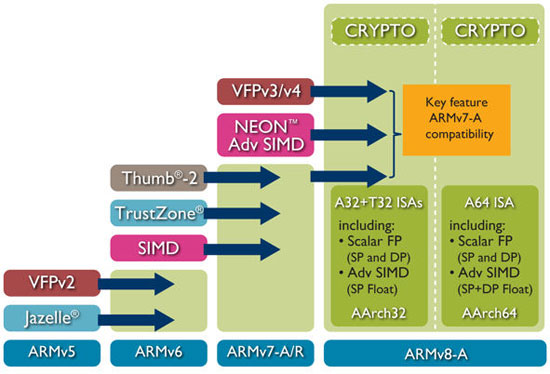
\includegraphics[width=0.7\textwidth]{./arm_arch.jpg}
\caption{Evolution of the ARM architecture}
\label{Evolution of the ARM architecture}
\end{figure}

\begin{packed_item}
	\item \textbf{ARMv5}: support for digital signal processing (DSP) algorithms and the Jazelle� Java byte code engine to enable hardware execution of Java bytecodes, thus improving performance of applications written in Java
	\item \textbf{ARMv6}: introduction of the SIMD (Single Instruction Multiple Data) technology. This extension is particularly used in audio and video processing. In addition a security extension has been introduced known as TrustZone. The Thumb-2 mode has also been introduced to improve code density and performance
	\item \textbf{ARMv7}: this architecture delivers a set of profiles customized to target applications. All Cortex processors implement the ARMv7 architecture, (except Cortex M0 and Cortex M1 series which implement ARMv6M):
	\begin{packed_item}
		\item \textbf{Cortex A}: Application profile implementing a virtual memory system architecture based on an MMU (memory management unit). An optional NEON processing unit for multimedia applications and advanced hardware Floating Point unit can be added
		\item \textbf{Cortex R}: Realtime profile implementing a protected memory system architecture based on an MPU (memory protection unit)
		\item \textbf{Cortex M}: Microcontroller profile designed for fast interrupt processing and ideal for cost-sensitive devices requiring highly deterministic behaviour
	\end{packed_item}
	\item \textbf{ARMv8}: ARMv8 introduces a 64-bit architecture support. The main feature addded is the instruction level support for cryptography
\end{packed_item}


\begin{figure}[h!]
\centering
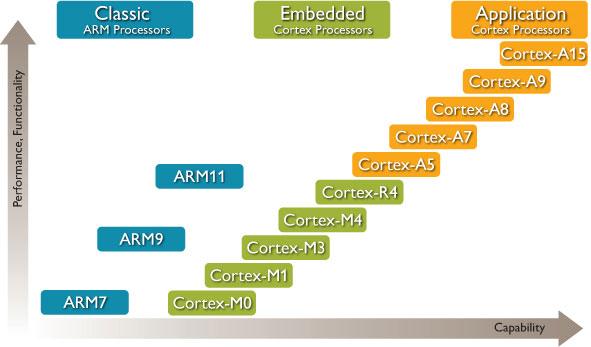
\includegraphics[width=0.7\textwidth]{./arm_proc.jpg}
\caption{ARM processors}
\label{ARM processors}
\end{figure}

\newpage

\section{Mbed}
Aiming to pursue new areas of expertise, ARM founded Mbed in 2009. Mbed's core area is the development of prototyping boards (called mbed) based on ARM processors (Cortex M0 and Cortex M3). Their purpose is to make simple and easy to setup prototyping solutions using 32-bit processors. Mbeds boards have been designed for quick experimentation; users can try something and see if it is doable in a very quick and easy manner.

\begin{figure}[h!]
\centering
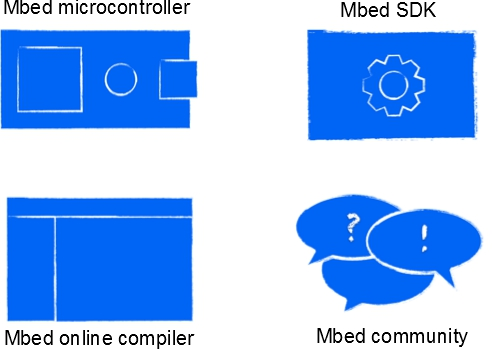
\includegraphics[width=0.5\textwidth]{./mbed_4elements.jpg}
\caption{Four main elements of Mbed}
\label{Four main elements of Mbed}
\end{figure}

\subsection{Mbed boards: LPC1768 and LPC11U24}
For the moment, two boards have been designed. The first is based on the LPC1768 microcontroller from NXP which uses a Cortex M3:
\begin{packed_item}
	\item 96 MHz, 32 Kb of RAM, 512 Kb of flash
	\item 3 UART, 2 SPI, 2 I2C, 6 PWM, 6 ADC, GPIO, Ethernet, USB Host/Device
\end{packed_item}

\begin{figure}[htp]
  \centering
  \subfigure[mbed lpc1768 (Cortex M3)]{\label{fig:edge-a}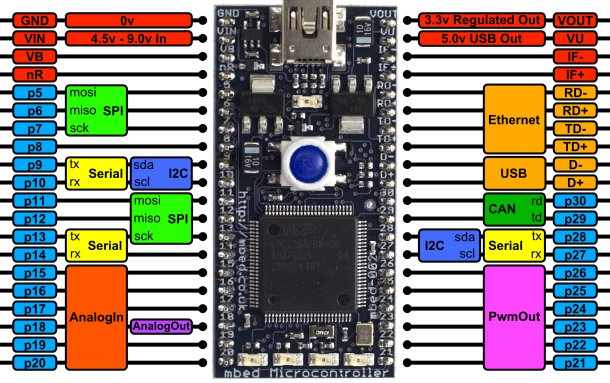
\includegraphics[scale=2.7]{./lpc1768.jpg}}                
  \subfigure[mbed lpc11U24 (Cortex M0)]{\label{fig:contour-b}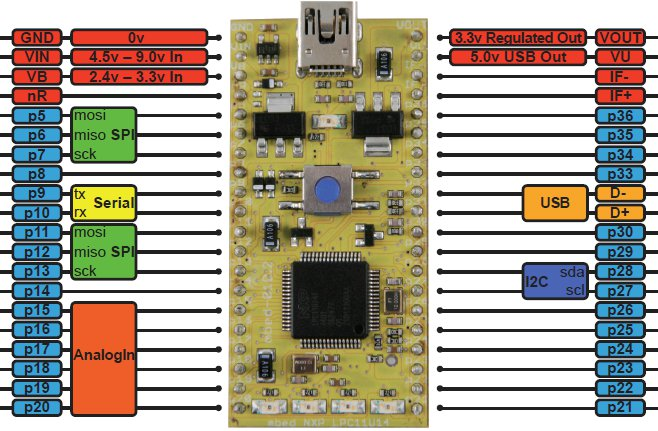
\includegraphics[scale=0.3]{./lpc11U24.jpg}} \\
  \caption{Mbed boards}
  \label{fig:contour}
\end{figure}

More recently, a new board based on a LPC11U24 (Cortex M0) was introduced. This mbed has been designed to prototype USB devices or battery powered applications:
\begin{packed_item}
	\item 48 MHz, 8 Kb of RAM, 32 Kb of flash
	\item UART, I2C, 2 SPI, 6 ADC, GPIO, USB Device
\end{packed_item}


Both mbed boards have a built-in USB drag and drop FLASH programmer. This feature allows mbed users to drag and drop a binary into the mbed, recognized as a USB mass storage device by a computer. It is very convenient and simple to flash a new program into the mbed:
\begin{packed_item}
	\item create a program (online IDE or offline toolchains)
	\item copy the binary generated into the mbed 
	\item press the reset button
\end{packed_item}


\subsection{The online compiler}
The two main keywords of Mbed are "simple" and "cloud computing". Users can use an online compiler to develop their programs in C++. They compile online and transfer the generated binary into the mbed, which is connected to a computer over a USB cable. They just have to press the reset button to see their program running.
\\

The online IDE is totally independent from the underlying operating system. It contains a lot of interesting features:
\begin{packed_item}
	\item Code editing with syntax highlighting and automatic indentation
	\item Multiple programs
	\item Import programs from online catalogue of published programs
	\item Import programs from zip file
	\item Full output of compile-time messages
	\item Multiple target support
	\item Publish your code directly from the compiler
	\item Export your programs as a .zip file
	\item Build information including graphical display of code size and RAM usage
	\item Import and update of libraries from SVN
	\item Version control: you can commit, revert, update, merge your programs
\end{packed_item}

\subsection{Mbed libraries}
In addition to the online compiler, almost all drivers have been implemented. Users just have to instantiate an object such as SPI or I2C to have access to an API which abstracts all the low-level layers. The figure~\ref{mbed libraries} shows on the left hand side all drivers implemented which are accessible over a C++ class. On the right hand side, a description, some basic examples and the API of a specific class can be found. Users can code using meaningful abstract objects and API calls, so there is no need to learn the microcontroller hardware details to get going.\\


\begin{figure}[h!]
\centering
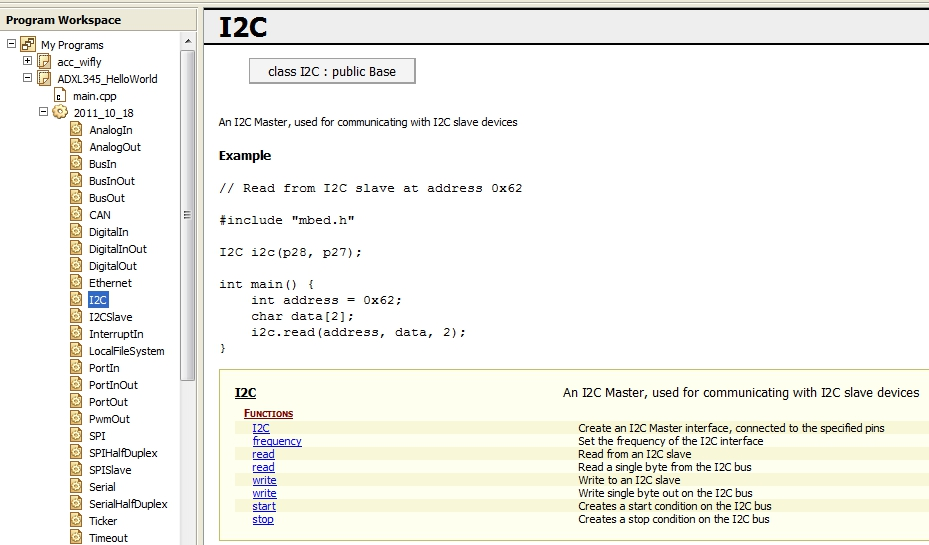
\includegraphics[width=0.8\textwidth]{./libraries.jpg}
\caption{mbed libraries}
\label{mbed libraries}
\end{figure}


\subsection{Mbed website: \textit{http://mbed.org/}}
Finally, users can access the mbed \textbf{forum} to troubleshoot their programs or ask questions. They also have a \textbf{handbook} where there is a lot of documentation and examples concerning mbed libraries or the hardware part of the mbed. However, I find that the most important and useful part of the website is the \textbf{cookbook}. The cookbook is a great source of examples contributed from, and edited by, other mbed users. You can almost always find a library to use with popular peripherals like accelerometers, pressure sensors... The user is free to contribute to this part of the website by writing articles explaining their project and code. 

\begin{comment}
\begin{figure}[h!]
\centering
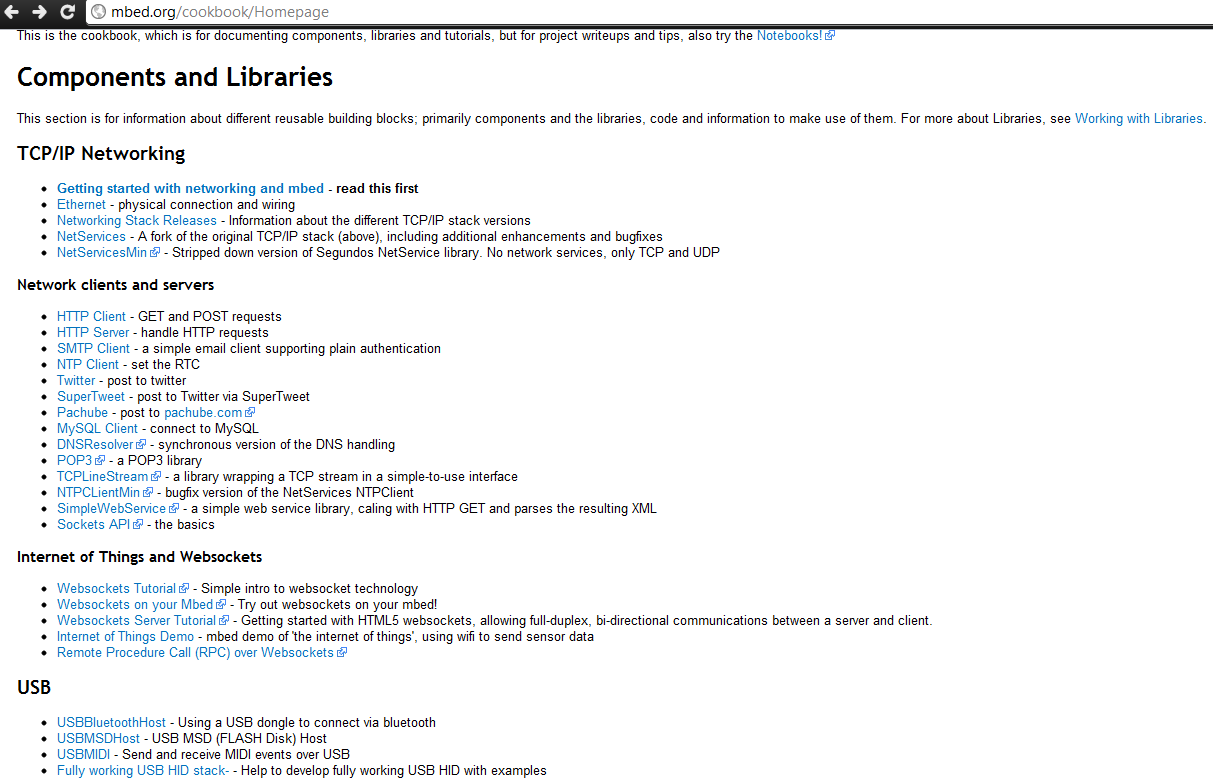
\includegraphics[width=1.0\textwidth]{./cookbook.jpg}
\caption{mbed cookbook}
\label{mbed cookbook}
\end{figure}
\end{comment}


\chapter{Internet Of Things: HTML5 on embedded systems}
Nowadays, an increasing number of devices is connected to the Internet. These devices include not only personal computers, but also mobile phones and digital televisions, etc.
Cisco predicted in an interview with the BBC that the number of internet connected devices is set to explode in the next four years to over 15 billion, twice the world's population, by 2015. Cisco is not the only company to predict a such boom; VMware's CEO Paul Maritz said during a speech at the 2011 VMworld conference in Las Vegas that:

\begin{quote} "Three years ago over 95 percent of the devices connected to the Internet were personal computers. Three years from now that number will probably be less than 20 percent. More than 80 percent of the devices connected to the Internet will not be Windows-based personal computers." \\
\end{quote}

Thus, the development and progress of technologies connecting different sensors and devices to the Internet is becoming ever more important. I will describe in this chapter two projects I took part in concerning the Internet of Things: connecting sensors to the cloud and Remote Procedure Call mechanism. Both of these projects use a new feature of HTML5: a WebSocket communication.


\begin{figure}[h!]
		\centering
		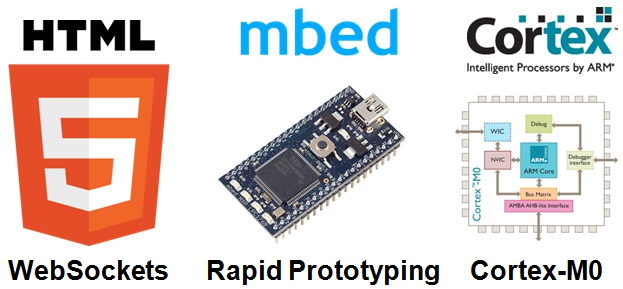
\includegraphics[width=0.5\textwidth]{./logo_ws.jpg}
		\caption{HTML5 on embedded systems}
		\label{HTML5 on embedded systems}
\end{figure}

\section{WebSockets}
\subsection{Introduction}
The HTML5 WebSocket specification defines a full-duplex single socket connection over which messages can be sent between client and server. The WebSocket standard simplifies much of the complexity around bi-directional web communication and connection management. Furthermore, it reduces polling and unnecessary network throughput overhead.

\subsection{Why the need for Websockets?}
Traditionally, when a web browser loads a webpage, it follows these basic steps:

\begin{packed_item}
	\item Open a short-lived connection to a web server
	\item Send a request to the server
	\item The web server acknowledges this request and sends back the response
	\item Close the connection to the server
\end{packed_item}

This architecture was designed primarily for document retrieval, where web browsers load static web pages from web servers. A transaction is based on a request/response mechanism. However, more and more frequently web applications require realtime capabilities. Developers wanted a technology where the server can send data to a client without the need of a client request. This technique is called server push. First attempts to provide realtime web applications was based on polling or server push technology:
\begin{packed_item}
	\item \textbf{polling}: the browser sends HTTP requests at regular intervals and immediately receives a response. This is an intuitive solution but it's often inefficient because in the case that the server does not have data to send, unnecessary requests will be sent. As a result there is a waste of bandwidth and CPU time on both the client and the server
	\item \textbf{long polling}: a basic example is a XMLHttpRequest object with long polling: The client sends requests through a XMLHttpRequest Javascript object. After each response, the client "rearms" the polling by sending a new request. The server holds client requests open until it has data to send, thus reducing unnecessary requests. However, the request/response mechanism is not avoided. In situations where there is a large volume of messages, long polling results in a continuous loop of immediate polls. Another problem with this technique is that during the reconnection process the data on the page could be out of date and inaccurate
	\item \textbf{streaming}: The browser sends a request and the server sends and maintains an open response that is continuously updated and kept open. This is much more efficient than polling or long polling as no HTTP headers are sent during the streaming period. As a result, the network traffic is reduced. The downside of streaming is that it is still encapsulated in HTTP, so intervening HTTP proxies may choose to buffer the response, increasing the latency of the message delivery. Alternatively, the proxy server may be configured to disconnect HTTP connections that are kept open for a certain amount of time.
\end{packed_item}


\begin{figure}[h!]
		\centering
		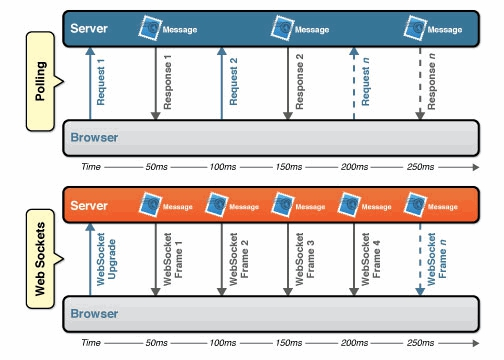
\includegraphics[width=0.7\textwidth]{./ws_poll.jpg}
		\caption{Latency and overhead comparison between polling and WebSocket applications \textit(Image courtesy of Kaazing)}
		\label{Latency and overhead comparison between polling and WebSocket applications}
\end{figure}

Ultimately, to provide full duplex communication on top of the HTTP half duplex architecture, many of today's solutions use two connections: one for the downstream and one for the upstream. The maintenance and coordination of these two connections introduces significant overhead in terms of resource consumption and increased complexity. WebSocket was developed to solve these issues. The new HTML5 feature provides interesting properties such as:
\begin{packed_item}
	\item a full duplex communication over a single TCP socket
	\item an overhead reduction
	\item less traffic: no need for polling
	\item proxy and firewall traversal: when a WebSocket detects the presence of a proxy, it issues an HTTP CONNECT to the proxy server to open a TCP/IP connection to a specific host and port
	\item standard and secure connections over ws:// and wss:// prefixes: A standard websocket URL can be: 
	\begin{center}
		\textbf{ws://example.com}
	\end{center}
\end{packed_item}

The figure~\ref{Latency and overhead comparison between polling and WebSocket applications} shows the reduction in latency. Once the connection is established, messages can flow between server and client. As the connection remains open, there is no need to send another request to the server.

\subsection{Websocket protocol}

To establish a WebSocket connection, the client and server upgrade from the HTTP protocol to the WebSocket protocol during their initial handshake. Another attractive aspect is their HTTP-compatible handshake. This means HTTP servers can share their default HTTP (80) and HTTPS (443) ports with a WebSocket server. After the handshake, a full TCP socket communication with a specific data framing is available. \\

The handshake from the client is as follows: \\

\fbox{\begin{minipage}{1.0\textwidth} \small
	GET /ws HTTP/1.1 \\
	Host: example.org \\
  Connection: Upgrade \\
  Sec-WebSocket-Key: dGhlIHNhbXBsZSBub25jZQ== \\
  Upgrade: WebSocket \\
  Origin: http://example.org \\
  Sec-WebSocket-Version: 13
  \end{minipage}
}
\\


The handshake from the server is as follows: \\

\fbox{\begin{minipage}{1.0\textwidth} \small
        HTTP/1.1 101 Switching Protocols \\
        Upgrade: websocket \\
        Connection: Upgrade \\
        Sec-WebSocket-Accept: s3pPLMBiTxaQ9kYGzzhZRbK+xOo=
        \end{minipage} 
        } \\


Once the Websocket connection is established, data can be exchanged between client and server. Data can either be text frame encoded as UTF-8 or binary data. Main fields of the data framing represented on the figure~\ref{Websocket data framing} are:

\begin{figure}[h!]
		\centering
		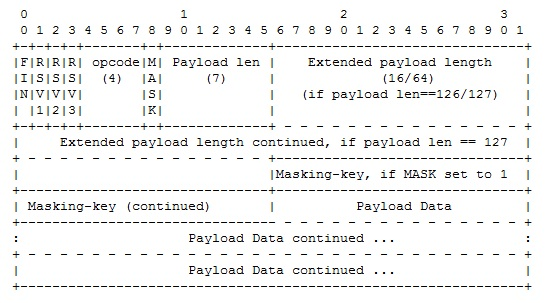
\includegraphics[width=0.7\textwidth]{./frame_ws.jpg}
		\caption{WebSocket data framing}
		\label{WebSocket data framing}
\end{figure}

\begin{packed_item}
	\item FIN: Indicates that this is the final fragment in a message.
	\item RSVx: reserved (0)
	\item Opcode: meaning of the payload:
		\begin{packed_item}
			\item 0x0: continuation frame
			\item 0x1: text frame (the payload is text data encoded as UTF-8)
			\item 0x2: binary frame (the payload is binary data)
			\item 0x8: connection close
			\item 0x9: ping (can be used as keep-alive mechanism)
			\item 0xa: pong (can be used as keep-alive mechanism)
		\end{packed_item}
	\item Mask: defines whether the payload data is masked or not
	\item payload length (in bytes):
		\begin{itemize}
			\item 0 - 125: payload length
			\item 126: the following 2 bytes represent the payload length
			\item 127: the following 8 bytes represent the payload length
		\end{itemize}
	\item Masking-key: used to unmask the payload
	\item Payload data: data
\end{packed_item}


\subsection{Architecture of a WebSocket communication}
WebSocket communications may involve several clients connected to the same WebSocket server. All messages from browsers are sent to the server, where the server manages them. It can, for instance, decide to send a message received from one client to another, or to broadcast all messages received to all clients connected.


\begin{figure}[h!]
		\centering
		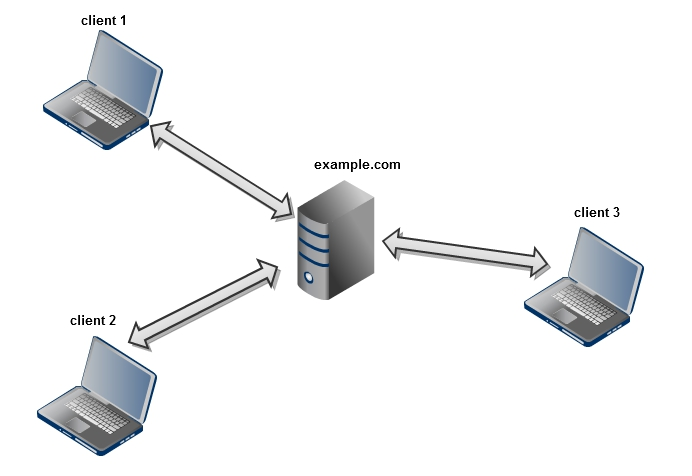
\includegraphics[width=0.6\textwidth]{./ws.jpg}
		\caption{Example of WebSocket communication}
		\label{Example of WebSocket communication}
\end{figure}

For example, let's say that there is an existing WebSocket server: \textbf{example.com} which is listening on port 80. A client can open a connection, receive and send messages to this server with these few lines of javascript:

\begin{center}
\begin{lstlisting}[label=Javascript Websocket Hello World,caption=Javascript Websocket Hello World]
var ws = new WebSocket("ws://example.com");
ws.onopen = function(evt) { 
   alert("Connection open"); 
   ws.send("Hello")}; 
};
ws.onmessage = function(evt) { 
   alert( "Message received: " + evt.data); 
}; 
ws.onclose = function(evt) { 
   alert("Connection closed."); 
};
\end{lstlisting}
\end{center}


\subsection{The mbed WebSocket library}
A WebSocket client library has been developed in order to exchange data between an mbed and a server over a WebSocket communication. The library can be used over an ethernet connection, or a wifi connection using a Roving Networks wifly module. The library uses existing libraries such as the wifi module library or the TCP socket library, part of the TCP/IP stack (port of lwIP for mbed). For instance, the method which connects an mbed to a WebSocket server over wifi is:


\begin{center}
\begin{lstlisting}[label=Connection to a WebSocket server,caption=Connection to a WebSocket server]
// open a socket on a specific port
sprintf(cmd, "open %s %s\r\n", ip_domain.c_str(), port.c_str());
wifi->send(cmd, "OPEN");

//send WebSocket HTTP header
sprintf(cmd, "GET /%s HTTP/1.1\r\n", path.c_str());
wifi->send(cmd);
sprintf(cmd, "Host: %s:%s\r\n", ip_domain.c_str(), port.c_str());
wifi->send(cmd);
wifi->send("Upgrade: WebSocket\r\n");
wifi->send("Connection: Upgrade\r\n");
wifi->send("Sec-WebSocket-Key: dGhlIHNhbXBsZSBub25jZQ==\r\n");
sprintf(cmd, "Origin: http:%s:%s\r\n", ip_domain.c_str(), port.c_str());
wifi->send(cmd);
if (!wifi->send("Sec-WebSocket-Version: 13", "s3pPLMBiTxaQ9kYGzzhZRbK+xOo="))
   return false;

\end{lstlisting}
\end{center}







\newpage









\section{Connecting sensors to the cloud}
Mbed wanted to demonstrate that it was possible to access sensor data all over the world using an mbed board and HTML5 WebSockets. For this, two prototype boards have been developed with different sensors:

\begin{packed_item}
	\item \textbf{accelerometer board} with a three axis accelerometer
	\item \textbf{environmental board} with:
		\begin{packed_item}
			\item light sensor
			\item pressure sensor
			\item microphone
		\end{packed_item}
\end {packed_item}

The idea behind this project is that the sensor data has to be available everywhere as quickly as possible. That's why we wanted to involve smartphones connected to the Internet over 3G. To achieve this, we used QR (Quick Response) codes. A QR code is a type of matrix-barcode and encodes information. For this project, all QR codes encode URL(s) of webpages which receive the sensor data. Each board has a different QR code. The steps to access data for a user are:

\begin{packed_item}
	\item Place the objects (mbed, sensors, QR code associated to this board) where desired
	\item Scan the QR code with a smartphone, access the webpage associated and see the sensor data displayed
	\item The graph can then be added to a central \textbf{dashboard}
\end{packed_item}

\begin{figure}[h!]
		\centering
		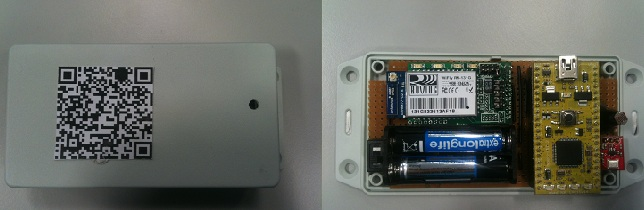
\includegraphics[width=0.8\textwidth]{./env_board_qr.jpg}
		\caption{Environmental board with its QR code}
		\label{Environmental board with its QR code}
\end{figure}

\begin{figure}[h!]
		\centering
		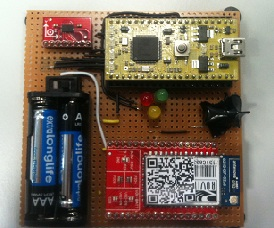
\includegraphics[width=0.4\textwidth]{./acc_board.jpg}
		\caption{Accelerometer board with its QR code}
		\label{Accelerometer board with its QR code}
\end{figure}



\subsection{Architecture: mbed boards, WebSocket server, browsers}
We can distinguish two different parts:
\begin{packed_item}
	\item a WebSocket server
	\item all clients connected to the server:
	\begin{packed_item}
		\item mbed boards
		\item browsers:
		\begin{packed_item}
			\item \textbf{smartphone webpages}: displays a unique graph containing sensor data of a specific board. This webpage is accessed by reading the QR code associated to the board. A user can then decide to \textbf{add} or \textbf{remove} this graph to or from a central dashboard
			\item \textbf{dashboard}: central webpage showing graphs of different boards added by users
		\end{packed_item}
	\end{packed_item}
\end{packed_item}

All mbed boards send messages in JSON (JavaScript Object Notation) format to the WebSocket server containing sensor data. A JSON object is an unordered collection of key:value pairs with the ':' character separating the key and the value. The following example shows a basic JSON message:
\begin{lstlisting}[label=JSON message example,caption=JSON message example]
{
     "id"     : "acc_board",
     "acc_x"  : 250,
     "acc_y"  : 15,
     "acc_z"  : 100
}
\end{lstlisting}

The WebSocket server broadcasts all messages received to all clients connected. In particular, browsers are able to receive data from sensors. They can then ignore or not the messages received.

\begin{figure}[h!]
		\centering
		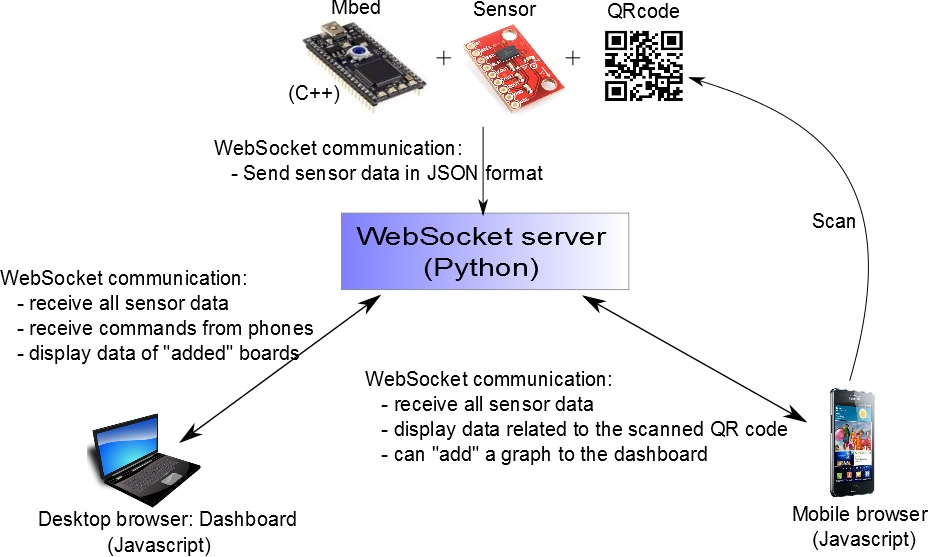
\includegraphics[width=0.8\textwidth]{./ws_arch.jpg}
		\caption{Connecting sensors to the cloud project architecture}
		\label{Connecting sensors to the cloud project architecture}
\end{figure}


\subsection{WebSocket server: Tornado}
The WebSocket server used for this project is based on the Tornado Framework. This framework is written in Python, and it's a non blocking web server. It uses \textbf{epoll} which permits  handling thousands of connections. Some interesting features are, for instance:
\begin{packed_item}
	\item http server
	\item template language
	\item mySQL client wrapper
	\item WebSocket server
\end{packed_item}

\begin{lstlisting}[label=Launching of an HTTP server with Tornado,caption=Launching of an HTTP server with Tornado]
application = tornado.web.Application([
    (r'/ws/(.*)/(.*)', WSHandler),
], **settings)

if __name__ == "__main__":
    http_server = tornado.httpserver.HTTPServer(application)
    http_server.listen(80)
    tornado.ioloop.IOLoop.instance().start()
\end{lstlisting}

The previous lines launch a http server associated with a class (WSHandler). All requests having a path matching the regular expression \textbf{/ws/*/*} will be processed by WSHandler. The first argument of the path represents a channel and the second one the connection mode. This means that to open a connection with this server, a client has to join the server at the address: 
\begin{center}
\textbf{ws://sockets.mbed.org/ws/\textless{}channel\textgreater{}/\textless{}mode\textgreater{}}
\end{center}

The WebSocket server is divided into channels. All clients can send and receive messages over a same channel. However, each client can choose its connection mode:

\begin{packed_item}
	\item \textbf{write-only (wo)}: the client can write on a certain channel but cannot receive messages
	\item \textbf{read-only (ro)}: the client can read messages on a certain channel but cannot write messages
	\item \textbf{read-write (rw)}: the client can read and write messages over a channel
\end{packed_item}

When the server receives a message from a client in a certain channel, it will broadcast it to all clients connected to this channel which are in \textbf{rw} or \textbf{ro} mode. This mechanism is done in WSHandler which inherits from tornado.websocket.WebSocketHandler. The WebSocket protocol is implemented in the base class. Different methods can be overriden in WSHandler, called on different events:

\begin{packed_item}
	\item a connection has been opened
	\item a message is received
	\item a connection has been closed
\end{packed_item}

\begin{lstlisting}[label=Broadcast messages received,caption=Broadcast messages received]
class WSHandler(tornado.websocket.WebSocketHandler):
    def open(self, chan, mode):
        self.channel = chan
        self.mode = mode
        if mode == 'rw' or mode == 'ro' or mode =='wo':
            if not subscribers.get(self.channel):
                subscribers[self.channel] = []
            subscribers[self.channel].append(self)	
            logging.warning("New Subscribers: chan %s, mode: %s"%(chan, mode))

    def on_message(self, message):
        for client in subscribers.get(self.channel, []):
        		if client.mode != 'wo':
	              client.write_message(message)
\end{lstlisting}



\subsection{Mbed boards}
\subsubsection{Hardware}

\begin{figure}[h!]
		\centering
		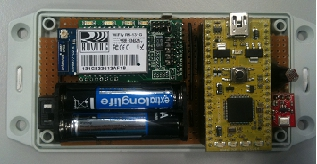
\includegraphics[width=0.5\textwidth]{./env_board.jpg}
		\caption{Environmental board}
		\label{Environmental board}
\end{figure}

The hardware is very simple to setup as mbed has been designed with quick prototyping in mind. The main parts are:
\begin{packed_item}
	\item one mbed
	\item a wifi module
	\item sensors
\end{packed_item}

A wifi module has been chosen to connect the mbed to the internet and access the WebSocket server. I wanted a wifi module easy to use and easy to connect to the mbed. I chose a wifi module from Roving Networks which integrates a full TCP/IP stack. The communication between the mbed and the wifi module is established over a serial communication.

Concerning sensors, all are also very easy to use and to connect. The 3-axis accelerometer and the pressure sensor are connected to the mbed over SPI. Libraries for these sensors have already been developed by the mbed community. The light sensor is connected over a GPIO, as is the microphone. 


\subsubsection{Software}
The program running on the mbed has to:
\begin{packed_item}
	\item connect to a network
	\item connect to the WebSocket server
	\item in a loop:
		\begin{packed_item}
			\item read sensor data
			\item send them over WebSocket to the server
		\end{packed_item}
\end{packed_item}


\begin{center}
\begin{lstlisting}[label=Streaming data code example,caption=Streaming data code example]
// wifly instance to connect the wireless network
Wifly wifly(p9, p10, p30, "network", "password", true);

// WebSocket instance to send sensor data to the WebSocket server: we use the channel "sensors" in write-only mode
Websocket ws("ws://sockets.mbed.org/ws/sensors/wo", &wifly);

int main() {
    char json_str[100];
    int press;
    double temp;
    int light;
    unsigned short mic;
    
    // join the wireless network
    wifly.join();
    		
    // connection to the WebSocket server
    ws.connect();
    		
    while (1) {
      wait(0.1);

      //pressure
      press = scp1000.readPressure();

      //temperature
      temp = scp1000.readTemperature();

      //light
      light = light_pin.read_u16()/480;

      //microphone
      mic = readMicrophone();

      //format data in a JSON string and sent it
      sprintf(json_str, "{\"id\":\"wifly_env\",\"p\":%d,\"t\":%d,\"l\":%d,\"m\":%d}", (int)press, (int)temp, (int)(light), mic);
      ws.send(json_str);
   }
}
\end{lstlisting}
\end{center}



\subsection{Browsers}
In the process of developing clean and minimalist webpages for computer and smartphone use, I needed a graph that scrolled smoothly in real time. For this, I chose to use another new HTML5 feature, the canvas element. Javascript code can access this drawable region through a complete API. The canvas element can be for instance used to display realtime graphs or to build games and animations.
\\


There are two different webpages:
\begin{packed_item}
	\item \textbf{smartphone webpages}: display only the graphed data from the corresponding devices, added via QR code. Two buttons can be used to add or remove a specific graph from the dashboard webpage
	\item \textbf{dashboard}: display all graphs added by users
\end{packed_item}

\subsubsection{Realtime graphs}
I used Smoothie Charts which is a javascript library to stream data using a canvas element. Smoothie Charts is a small charting library designed for live streaming data. The idea is to display in realtime sensor data in a chart refreshed everytime that we receive a new data.

\subsubsection{A QR code associated to each mbed board}
A smartphone has to scan a QR code to access sensor data of a specific board. The difference between all mbed boards is made over a variable passed to a PHP webpage:
\begin{packed_item}
	\item \textbf{accelerometer board}: sensors.php?id=wifly\_acc
	\item \textbf{environmental board}: sensors.php?id=wifly\_env
\end{packed_item}

According to the parameter, a smartphone webpage will then listen only messages from a specific board.

\subsubsection{WebSocket and JSON messages exchanged}
Several messages are exchanged between clients and server. 
\begin{packed_item}
	\item from mbed boards: 
		\begin{center}
				\{"id"="wifly\_acc", "ax"=x\_axis\_value, "ay"=y\_axis\_value, "az"=z\_axis\_value\} \\
				\{"id"="wifly\_env", "l"=light\_value, "t"=temperature\_value, "p"=pressure\_value, "m"=microphone\_value\}
		\end{center}
	\item from smartphones:
		\begin{center}
				\{"id"="acc\_add"\} \\
				\{"id"="env\_add"\} \\
				\{"id"="acc\_clean"\} \\
				\{"id"="env\_clean"\}
		\end{center}
		
\end{packed_item}

Messages sent by mbed boards to the server contain sensor data. When a client receives such a message broadcasted by the server, it can refresh a realtime graph showing the sensor data against time. \\

Messages sent by smartphones to the server control graphs on the dashboard webpage. For instance, if a user scans the QR code of the accelerometer board and presses the add button, the message 
		\begin{center}
				\{"id"="acc\_add"\}
		\end{center}
is sent to the server. The server broadcasts it. In particular, the dashboard receives it and displays the corresponding graph. \\

\subsubsection{Architecture of webpages}
The architecture of smartphone webpages is quite simple:

\fbox{\begin{minipage}{1.0\textwidth}
\begin{packed_item}
	\item Connection to the WebSocket server
	\item When a message is received:
		\begin{packed_item}
			\item check the validity of the message
			\item if the message is a request to add a graph on a dashboard:
			\begin{packed_item}
				\item ignore it
			\end{packed_item}
			\item if the message is coming from a board:
					\begin{packed_item}
						\item if the \textbf{id field} matches the argument passed to the PHP webpage, refresh the graph
						\item otherwise, ignore the message
					\end{packed_item}
		\end{packed_item}
\end{packed_item}
\end{minipage} 
} \\

The architecture of the dashboard is a little more complicated because it has to take into account messages from boards and from smartphones:

\fbox{\begin{minipage}{1.0\textwidth}
\begin{packed_item}
	\item Connection to the WebSocket server
	\item When a message is received:
		\begin{packed_item}
			\item check the validity of the message
			\begin{packed_item}
				\item if the message is a request to add a graph on a dashboard:
				\begin{packed_item}
					\item update the Document Object Model (DOM) using the jQuery javascript library
					\item display the graph associated to this request
				\end{packed_item}
				\item if the message is coming from a board:
				\begin{packed_item} 
					\item if the board has been previously added, refreshes a specific graph according to the \textbf{id field}
				\end{packed_item}
			\end{packed_item}
		\end{packed_item}
\end{packed_item}
\end{minipage} 
} \\


\begin{center}
\begin{lstlisting}[label=Manipulation of WebSocket messages by the dashboard,caption=Manipulation of WebSocket messages by the dashboard]
    //WebSocket instance connected on the same subnetwork as the mbed boards
    websocket = new WebSocket('ws://sockets.mbed.org/ws/sensors/rw');

    websocket.onmessage = function (evt) {
			var json_sensor = jQuery.parseJSON(evt.data.toString());
			date = new Date().getTime();
			if(json_sensor.id == "wifly_acc") 
			{
				acc_x.append(date, json_sensor.ax);
				acc_y.append(date, json_sensor.ay);
				acc_z.append(date, json_sensor.az);

				refreshBall();
			}
			else if(json_sensor.id == "wifly_env") 
			{
				light.append(date, json_sensor.l);
				temp.append(date, json_sensor.t);
				press.append(date, json_sensor.p / 1000);
				mic.append(date, json_sensor.m);

				refreshEnv();
			}
			else
				manipulateDOM(json_sensor.id);
		};
	\end{lstlisting}
\end{center}

As expected, when a WebSocket message is received the corresponding graph is updated. If the \textbf{"id"} field on the message is different from \textbf{wifly\_acc} or \textbf{wifly\_env}, it's probably a message coming from a smartphone indicating to the dashboard to display or not a specific graph. 

\subsubsection{Results}

On the dashboard, we can see that the environmental board and the accelerometer have been added:
\begin{packed_item}
	\item realtime graph available (10 Hz): light, pressure, temperature, microphone and accelrometer data
	\item more information are available on the right: other representations of sensor data
\end{packed_item}

On the smartphone webpage, we can observe the live graph containing sensor data only from the accelerometer board. On this webpage, we can manage the dashboard with the "add" and "clear" buttons.
\newpage

\begin{figure}[h!]
		\centering
		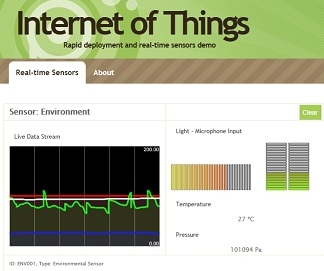
\includegraphics[width=0.6\textwidth]{./dashboard.jpg}
		\caption{Dashboard webpage}
		\label{Dashboard webpage}
\end{figure}

\begin{figure}[h!]
		\centering
		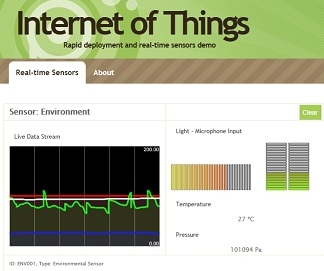
\includegraphics[width=0.6\textwidth]{./dashboard.jpg}
		\caption{Smartphone webpage containing accelerometer data}
		\label{Smartphone webpage containing accelerometer data}
\end{figure}



\newpage

\section{Remote Procedure Call over WebSockets}
After having connected sensors to the Internet and demonstrated the power of HTML5 in embedded systems, mbed wanted to use WebSockets to design an RPC (Remote Procedure Call) mechanism. The idea is to enable users to call a specific method on a specific mbed. All mbeds are connected to the Internet.

\subsection{Architecture: mbed boards, WebSocket server}

\begin{figure}[h!]
		\centering
		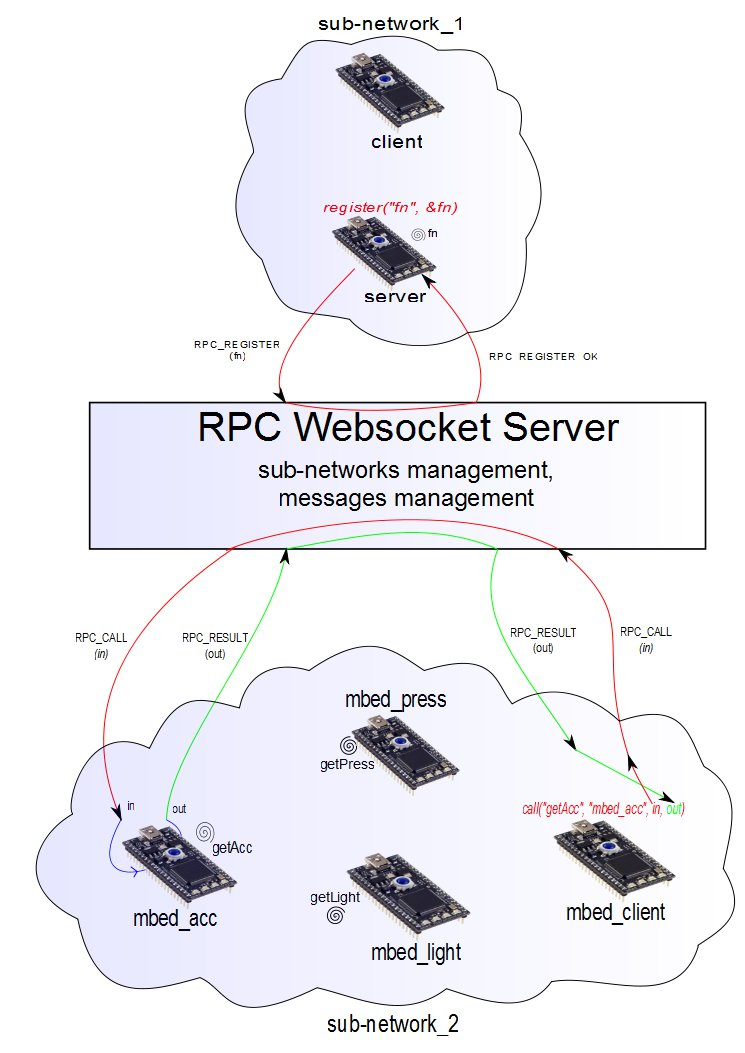
\includegraphics[width=0.7\textwidth]{./rpc-1.jpg}
		\caption{RPC architecture}
		\label{RPC architecture}
\end{figure}

The figure~\ref{RPC architecture} distinguishes two main elements:
\begin{packed_item}
	\item \textbf{Two different subnetworks}. On each subnetwork, all mbeds can share methods or execute a non-local one
	\item \textbf{An RPC WebSocket server} which is responsible for managing all subnetworks and all messages exchanged. This server is written in Python and uses Tornado
\end{packed_item}


Each mbed belongs to a specific subnetwork and is identified by a specific name. This identification is made over the URL used to connect to the WebSocket server as shown in the figure~\ref{RPC: mbed identification on a subnetwork}. \\

\begin{figure}[h!]
		\centering
		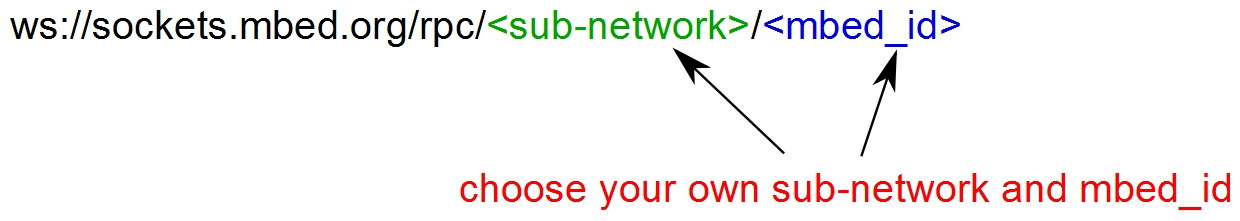
\includegraphics[width=0.7\textwidth]{./rpc_ws.jpg}
		\caption{RPC: mbed identification on a subnetwork}
		\label{RPC: mbed identification on a subnetwork}
\end{figure}

Different steps are required to execute a distant method:
\begin{packed_item}
	\item connect several mbeds to the same subnetwork over a WebSocket communication
	\item all mbeds can register methods: an mbed has to register one or more methods to the server before others can call them
	\item an mbed connected over the same subnetwork as the previous mbed can call the registered method
	\item the distant mbed executes the method and return the results
	\item the local mbed can then handle the result of the distant method
\end{packed_item}

\subsection{Protocol}
The RPC mechanism relies on JSON messages exchanged. On these messages, we need to specify:
\begin{packed_item}
	\item the \textbf{source} of the message
	\item the \textbf{destination} of the message
	\item the \textbf{message name}:
		\begin{packed_item}
			\item CALL: to call a distant function
			\item RESULT: this message contains the result of a previous CALL
			\item REGISTER: used to register a specific method to the WebSocket server
			\item INFO\_METHODS: a client can have access to all methods registered from a specific client
			\item ERROR: an error has been detected
		\end{packed_item}
	\item the \textbf{message ID}: random number used to identify a transaction. For a valid RPC transaction, the request and the answer have to have the same message ID.
\end{packed_item}

The previous fields are common to all messages exchanged. After each message, other possible fields are:


\begin{packed_item}
	\item CALL:
		\begin{packed_item}
			\item \textbf{method}: distant method name which will be called
			\item \textbf{params}: parameters for this method
		\end{packed_item}
	\item RESULT:
		\begin{packed_item}
			\item \textbf{result}: result of the function called remotely
		\end{packed_item}
	\item REGISTER:
		\begin{packed_item}
			\item \textbf{fn}: on the network, a distant method will be identified by this field
		\end{packed_item}
	\item ERROR:
		\begin{packed_item}
			\item \textbf{cause}: cause of the error:
			\begin{packed_item}
				\item JSON\_PARSE\_ERROR: error in the json format
				\item JSON\_RPC\_ERROR: error in the rpc message format
				\item METHOD\_NOT\_FOUND: the distant method called has not been registered
				\item CLIENT\_NOT\_CONNECTED: the client which must execute the distant method is not connected
			\end{packed_item}
		\end{packed_item}
\end{packed_item}

\subsection{Signature of methods handled}
A user wants to be able to register and then call a function of his choice. So a function can take all kinds of input arguments and return whatever type. The solution is to convert several types of argument into a more generic object called MbedJSONValue. This class can handle parameters such as:
\begin{packed_item}
	\item booleans
	\item integers
	\item doubles
	\item strings
	\item arrays of MbedJSONValue
	\item MbedJSONValue object inside another one
\end{packed_item}

As messages are exchanged in JSON format, I decided to use a JSON parser/serializer to convert a MbedJSONValue into a JSON string and vice-versa. It is based on the tiny picojson library. A unique signature can then be defined to be handled by the RPC mechanism:

\begin{center}
\textbf{void fn(MbedJSONValue\& in, MbedJSONValue\& out)}
\end{center}

The manipulation and creation of MbedJSONValue can be done very easily as shown on this example:

\begin{lstlisting}[label=MbedJSONValue manipulation,caption=MbedJSONValue manipulation]
 #include "mbed.h"
 #include "MbedJSONValue.h"
 #include <string>

 int main() {     
    MbedJSONValue demo;

    const  char * json = "{\"my_array\": [\"demo_string\", 10], \"my_boolean\": true}";

    //parse the previous string and fill the object demo
    parse(demo, json);

    std::string my_str;
    int my_int;
    bool my_bool;

    my_str = demo["my_array"][0].get<std::string>();
    my_int = demo["my_array"][1].get<int>();
    my_bool = demo["my_boolean"].get<bool>();
   
    printf("my_str: %s\r\n", my_str.c_str());
    printf("my_int: %d\r\n", my_int);
    printf("my_bool: %s\r\n", my_bool ? "true" : "false");
 }
   \end{lstlisting}

\subsection{Core of the RPC mechanism: MbedJSONRpc}
\subsubsection{Register a method}
To register a method, a user has to invoke:
\begin{lstlisting}[label=Register a method,caption=Register a method]
template<typename T> RPC_TYPE registerMethod(const char * public_name, T * obj_ptr, void (T::*fn)(MbedJSONValue& val, MbedJSONValue& res))
\end{lstlisting}


This method is responsible for registering the specified method on the rpc WebSocket server and needs several steps:
\begin{packed_item}
	\item Send a WebSocket message to the server containing a MSG\_REGISTER request:
	\begin{packed_item}
		\item from: mbed\_id
		\item to: server
		\item msg: REGISTER
		\item fn: public\_name 
	\end{packed_item}
	\item Wait a response from the server (if the request is successful: REGISTER\_OK)
	\item Fill two local arrays:
	\begin{packed_item}
		\item callback: contains function pointers of methods registered
		\item name: contains identifiers of methods registered
	\end{packed_item}
\end{packed_item}


After this step, a distant mbed will be able to call the method registered identified by "public\_name".
    
\subsubsection{Call a registered method}
To call a distant method, a user has to invoke:
\begin{lstlisting}[label=Call a distant method,caption=Call a distant method]
RPC_TYPE MbedJSONRpc::call(const char * fn, const char * dest, MbedJSONValue& in, MbedJSONValue& out)
\end{lstlisting}

This method, in order to call a distant method, requires several steps:
\begin{packed_item}
	\item Serialize the in MbedJSONValue object in order to be sent over WebSocket
	\item Send a WebSocket message to the server containing a MSG\_CALL request
	\begin{packed_item}
		\item from: mbed\_id
		\item to: dest
		\item msg: CALL
		\item fn: fn
		\item params: "in" serialized
	\end{packed_item}
	\item Wait for a MSG\_RESULT message from the server containing the result of the distant method
	\item Convert the JSON string received in the "result" parameter into a MbedJSONValue
	\item Fill the "out" reference with the previous MbedJSONValue
\end{packed_item}

After this step, a user can handle the result of the distant method contained in the "out" reference.

\subsubsection{Listen for incoming request}
To listen incoming requests, a user has to invoke:
\begin{lstlisting}[label=Listen incoming requests,caption=Listen incoming requests]
void MbedJSONRpc::work()
\end{lstlisting}

This method does the following steps:
\begin{packed_item}
	\item Tries to read a WebSocket message
	\item If a message is available:
		\begin{packed_item}
			\item Check the validity of the message
			\item Convert the "params" field in a MbedJSONValue object
			\item Execute the registered method with the previous in argument. At the same time, the method will fill the "out" parameter containing the result
			\item Serialize the result of the method executed
			\item Send a MSG\_RESULT WebSocket message to the server;
			\begin{packed_item}
				\item from: mbed\_id
				\item to: msg["from"]
				\item msg: RESULT
				\item res: "out" parameter serialized
			\end{packed_item}
		\end{packed_item}
\end{packed_item}


\subsection{Mbed boards}
\subsubsection{Hardware}
The only requirement for the hardware is to have access to the internet so a wifi module or ethernet jack is required.

TODO: photo

\subsubsection{Software: mbed which registers a method}
I will demonstrate the program running on an mbed which has an accelerometer connected. The idea is to remotely access the accelerometer's values from another mbed.

\begin{lstlisting}[label=Client which registers a method,caption=Client which registers a method]

// accelerometer
ADXL345 accelerometer(p5, p6, p7, p8);

//wifi module
Wifly wifly(p9, p10, p17, "network", "password", true);

//WebSocket: configuration with subnetwork = sensor and mbed_id = mbed_acc 
Websocket webs("ws://sockets.mbed.org/rpc/sensor/mbed_acc",&wifly);

//RPC object attached to the WebSocket server
MbedJSONRpc rpc(&webs);

//Acc class. 
class Acc {
public:
    Acc() {};
    void getAcc(MbedJSONValue& in, MbedJSONValue& out) {
        int readings[3] = {0, 0, 0};
        accelerometer.getOutput(readings);
        out[0] = readings[0];
        out[1] = readings[1];
        out[2] = readings[2];
    }
};

//Instance of Acc. The method getAcc of this object will be registered
Acc acc;

int main() {
    RPC_TYPE t;
    
    //Accelerometers init
    accelerometer.init();
    
    //join the network
    wifly.join();
    
    //connect the WebSocket server
    webs.connect();

    //register the acc method and wait for incoming methods
    if((t = rpc.registerMethod("getAcc", &acc, &Acc::getAcc)) == REGISTER_OK) {
    		//wait for incoming CALL requests
    		rpc.work(); 
    }
    
}
\end{lstlisting}

\subsubsection{Software: mbed calling a distant method}

\begin{lstlisting}[label=Client which calls a distant method,caption=Client which calls a distant method]
//WebSocket over ethernet: configuration with subnetwork = sensor and mbed_id = mbed_acc
Websocket webs("ws://sockets.mbed.org/rpc/sensor/mbed_client");

//RPC object attached to the WebSocket server
MbedJSONRpc rpc(&webs);

int main() {
    RPC_TYPE t;
    
    //in: argument for the distant method (here empty)
    //out results of the distant method (accelerometers values)
    MbedJSONValue in, out;

		//connect the WebSocket server
    webs.connect();

    //CALL getAcc on mbed_acc
    if ((t = rpc.call("getAcc", "mbed_acc", in, out)) == CALL_OK) {
        printf("acc_x: %d\r\n", out[0].get<int>());
        printf("acc_y: %d\r\n", out[1].get<int>());
        printf("acc_z: %d\r\n", out[2].get<int>());
    }
}
\end{lstlisting}

\subsection{WebSocket server: Tornado}
The server uses the same framework used for the realtime streaming data project. It is responsible for managing all subnetworks and messages exchanged over a subnetwork. \\


The main data structure in order to represent the state of the whole network is a dictionary:
\begin{packed_item}
	\item Each key represents a specific subnetwork
	\item A value associated to a subnetwork is another dictionary:
		\begin{packed_item}
			\item Each key represents one mbed connected
			\item Each value is a dictionnary containing
			\begin{packed_item}
				\item a reference on the mbed
				\item an array containing methods registered by the mbed
			\end{packed_item}
		\end{packed_item}
\end{packed_item}


\begin{figure}[h!]
		\centering
		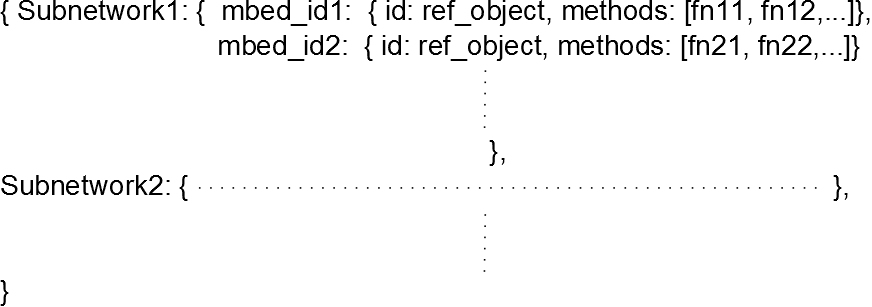
\includegraphics[width=0.6\textwidth]{./rpc_server_data_struct.jpg}
		\caption{Data structure for the RPC WebSocket server}
		\label{Data structure for the RPC WebSocket server}
\end{figure}


The WebSocket server does the following:
\begin{packed_item}
	\item If a new mbed connects a specific subnetwork:
	\begin{packed_item}
		\item Update the dictionary containing the network information by adding an entry to the subnetwork dictionary
	\end{packed_item}
	
	\item If the server receives a MSG\_REGISTER request:
	\begin{packed_item}
		\item Update the dictionary containing the network information by adding the new method to the array associated with the mbed
	\end{packed_item}
	
	\item If the server receives a MSG\_CALL request:
	\begin{packed_item}
		\item Check that the request comes from an mbed on the same subnetwork as the distant mbed
		\item Check that the method called is registered in the array associated to the called mbed
		\item If the two previous steps are sucessful, send a MSG\_CALL message to the distant mbed
	\end{packed_item}
	
	\item If the server receives a MSG\_RESULT message:
	\begin{packed_item}
		\item Check that the mbed which will receive the result of the distant method is on the same subnetwork
		\item Forward the message to the mbed which called the distant method
	\end{packed_item}
	
\end{packed_item}
	

\section{Conclusion}
For Mbed the Internet of Things is a very important field. We feel that in the future more and more devices will be connected to the cloud. Examples of applications could include:
\begin{packed_item}
	\item smart buildings
	\item medical devices
	\item factories
\end{packed_item}

The first project showed that it was possible to stream data sensor on realtime graphs accessible all over the world. The Remote Procedure Call project provides a mean to execute a method on a distant mbed. This can be useful, for instance, in critical places where the environment is inhospitable for humans. The common point of these two projects is the use of a WebSocket communication. This new way of communication enables realtime capabilities with a bidirectionnal communication between a client and server. It was quite interesting to develop projects using a protocol that was still in development. For instance, when I first started, the WebSocket data framing was not at all the same as now. It was much more simple: data frames started with 0x00 and ended with 0xff. The overhead was reduced but the final protocol defined in RFC 6455 provides more capabilities such as: raw binary can be sent, a ping/pong mechanism, a packet can be segmented. This change in the protocol led to tricky situations where the browser had been updated with the new protocol and the WebSocket server had not been. This resulted in the browser and the server being incompatible. For the moment, not all browsers are natively supporting WebSockets. Only Chrome 16 is supporting the last version of the protocol but we can hope that browsers will integrate this powerful feature soon.\\



After having worked on the Internet of Things, Mbed wanted to explore USB capabilities on the two mbed boards.
	
	
	
	
	
	
	
	
	
	

\chapter{Universal Serial Bus}

\section{Inside the USB bus}
\subsection{USB overview}
The Universal Serial Bus (USB) is the most widely used bus in today's computers. USB has particularly been designed to standardize connections between the computer and peripherals. For instance, keyboards, printers, scanners, disk drives or cameras can use the same bus to exchange data with a computer. USB has effectively replaced a variety of earlier interfaces, such as serial or parallel ports. The USB bus provides several benefits such as the same interface for many devices, the hot pluggable capability which allows a user to connect and disconnect a USB device whenever he wants, or the automatic configuration which is the capacity of the operating system to load a specific driver according to the device connected. Another useful benefit is that the USB interface provides power supply (5V) that can be used by a device so long as it doesn't require more than 500 mA.\\

USB version 1.0 supported two speeds, a full speed mode of 12Mbits/s and a low speed mode of 1.5Mbits/s. USB 2.0, which is the most widely version of USB, can reach 480Mbits/s. The 480Mbits/s is known as High Speed mode. USB version 3.0 specifies a maximum transmission speed of up to 5Gbits/s (known as SuperSpeed), but few products support USB 3.0 at present.
\\
\begin{table}[h!]
\begin{center}
\begin{tabular}{|l|l|l|}
\hline
\multirow{2}{*}{USB 1.0} & low-speed & 1.5Mbits/s \\
 & full-speed & 12Mbits/s \\ \hline
USB 2.0 & high-speed & 480Mbits/s \\ \hline
USB 3.0 & super-speed & 5Gbits/s \\ \hline
\end{tabular}
\end{center}
\caption{USB speeds}
\label{USB speeds}
\end{table}

The Universal Serial Bus is host controlled. However, there can only be one host per bus and the host is responsible for undertaking all transactions. Considering this restriction, two devices cannot exchange information without one being the host. Nevertheless, the On-The-Go specification, which is part of the USB 2.0 standard, has introduced a Host Negotiation Protocol, allowing two devices to negotiate for the role of host. With this specification, we can imagine a camera exchanging data with a printer without the need for a computer. 

\subsection{Topology}
The physical bus topology defines how USB devices are connected to the host. The USB network is implemented as a tiered star network with one host (master) and several devices (slaves). The topology looks like a tree. In order to increase the number of devices connected, a hub needs to be connected to the root port. This special hub and the root port are the first tier of the network. Furthermore, the USB network can support up to 127 external nodes but the number of tiers cannot exceed 7. The following diagram represents a possible connection architecture on a USB bus.


\begin{figure}[h!]
		\centering
		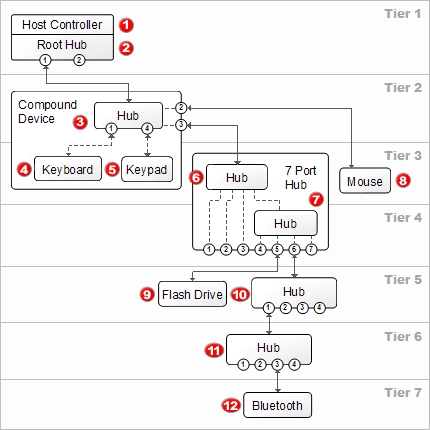
\includegraphics[width=0.4\textwidth]{./usb_topology.jpg}
		\caption{USB physical topology \footnotemark}
		\label{USB physical topology}
\end{figure}
\subsection{Endpoints and type of transfers}
Devices have a series of buffers to communicate with the host. Each buffer will belong to an endpoint. An endpoint is a uniquely identifiable entity on a USB device, which is the source or terminus of the data that flows from or to the device. For instance, the mbed based on a NXP LPC1768 microcontroller has 32 physical endpoints whereas the mbed based on the NXP LPC11U24, has 10 physical endpoints. One logical endpoint represents two physical endpoints. Each physical endpoint has a specific direction: either OUT to receive data from the host or IN to send data to the host. 


\footnotetext{reference: http://www.usblyzer.com}

\begin{figure}[h!]
		\centering
		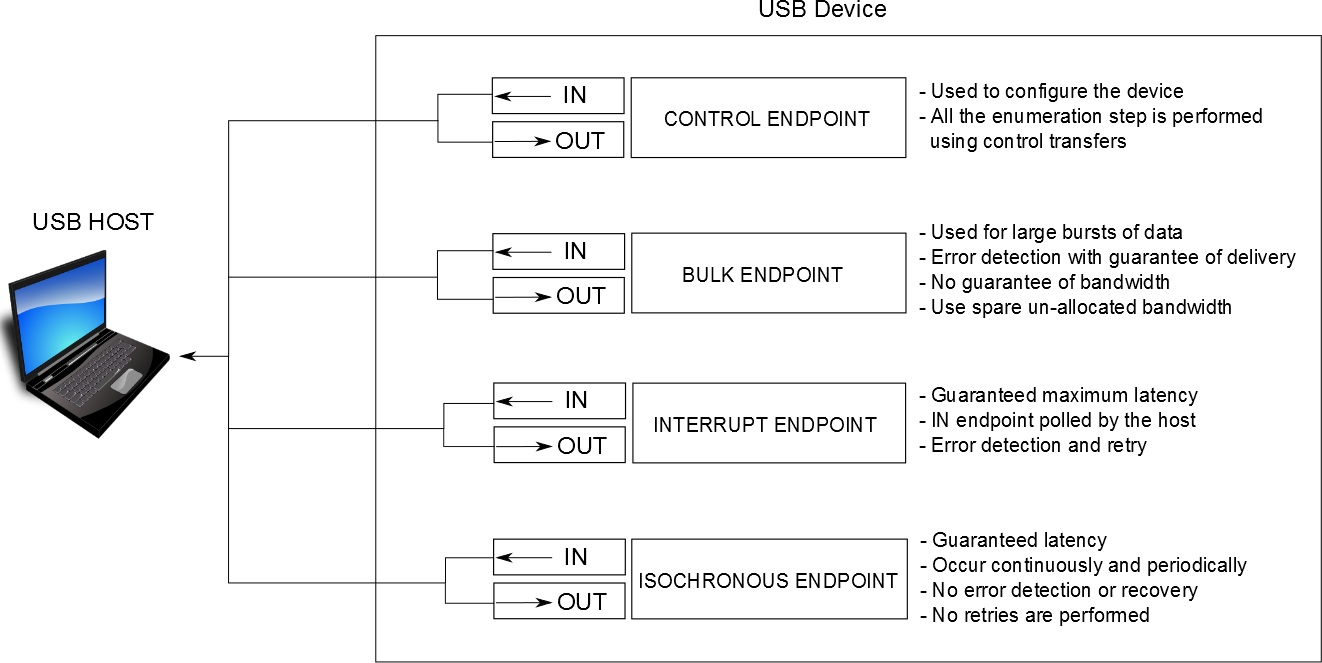
\includegraphics[width=0.8\textwidth]{./endpoints.jpg}
		\caption{Different types of endpoints}
		\label{Different types of endpoints}
\end{figure}

There are four types of endpoints which correspond to different requirements according to the device: 
\begin{packed_item}
	\item \textbf{Control endpoint}: All USB devices once connected perform an \textit{enumeration step} wherein the host requests all capabilities of the device. Control transfers are used to enumerate a device
	\item \textbf{Interrupt endpoints}: Interrupts transfers are used when a device requires responsiveness. Typical applications would include keyboard and mouse. Users don't want a noticeable delay between pressing a key or moving a mouse and seeing the result on the screen. An interrupt transfer only occurs when the host polls the device. There is a guarantee that the host will request a data within a specified time interval
	\item \textbf{Bulk endpoints}: Bulk transfers are typically used to transfer large amount of data like files to a printer. A bulk transfer uses spare un-allocated bandwidth, so time is not critical with bulk transfers. Typical applications include printers, scanners or mass storage devices
	\item \textbf{Isochronous endpoints}: Isochronous tranfers are used for streaming and realtime data. For instance, audio and video streaming devices use isochronous transfers. Such devices need a guaranteed delivery rate for data but if an error occurs, the data is not re-transmitted
\end{packed_item}
	

\subsection{Packets exchanged}
\subsubsection{\underline{Common fields in a USB packet}}

\begin{table}[h!]
\centering
\begin{tabular}{|c|c| >{\centering\arraybackslash}m{9cm} |}
\hline
Field & Length & Meaning \\ \hline
\multirow{2}{*}{SYNC} & low and full speed: 8bits  & \multirow{2}{9cm}{A packet starts with a SYNC pattern to allow the receiver bit clock to synchronise with the data.} \\
\cline{2-2}%
 & high speed: 32bits & \\ \hline
 
EOP &  & A packet ends with an End of Packet (EOP) field \\ \hline

PID & 8bits & Packet ID \\ \hline

\multirow{2}{*}{ADDR} & \multirow{2}{*}{7bits} & The address field specifies which device the packet is designated for\\ \hline

ENDP & 4bits & The endpoint number which the packet is designed for \\ \hline

\multirow{2}{*}{CRC} & \multirow{2}{*}{5 or 16bits} & Cyclic Redundancy Checks are performed on the data within the packet payload \\ \hline
\end{tabular}
\caption{Fields in a USB packet}
\label{Fields in a USB packet}
\end{table}

\subsubsection{\underline{Packets}}
\begin{packed_item}
	\item \textbf{Token Packet}: To indicate the type of transaction to follow, USB uses token packets:
		\begin{center}
		\begin{tabular}{|c|c|c|c|c|c|}
  	\hline
  		SYNC & PID & ADDR & ENDP & CRC5 & EOP \\ \hline
  		8/32bits & 8bits & 7bits & 4bits & 5bits &  \\
  	\hline
  	\end{tabular}
  	\end{center}
  	
  	There are three types of token packets: 
  	\begin{itemize} \itemsep 0em
			\item IN: The host wants to read information.
			\item OUT: The host wants to send information.
			\item SETUP: Used to begin control transfers.
  	\end{itemize}
  	
  	
	\item \textbf{Data Packet}: Packets which contain the payload
		\begin{center}
		\begin{tabular}{|c|c|c|c|c|}
  	\hline
  		SYNC & PID & DATA & CRC16 & EOP \\ \hline
  		8/32bits & 8bits & (0 - 1024) * 8bits & 16bits &   \\
  	\hline
  	\end{tabular}
  	\end{center}
  	
  	
	\item \textbf{Handshake Packet}: After a data stage, handshake packets are used to acknowledge data or to report errors
		\begin{center}
		\begin{tabular}{|c|c|c|}
  	\hline
  		SYNC & PID & EOP \\ \hline
  		8/32bits & 8bits &  \\
  	\hline
  	\end{tabular}
  	\end{center}
  	
  	There are four types of handshake packets:
  	\begin{itemize} \itemsep 0em
			\item ACK: Packet successfully received.
			\item NAK: The device temporary cannot send or received data
			\item STALL: Endpoint is halted, or control pipe request is not supported.
			\item NYET: No response yet from receiver (high speed only)
  	\end{itemize}
  	
  	
	\item \textbf{Start Of Frame Packet}: USB manages time in units called "frames" (USB 2.0 further added "microframes"), and uses frames/microframes to realize the concept of time. Each "frame" represents 1 ms, and each microframe represents 125 microseconds. When performing control, bulk or interrupt transfers with a peripheral device, there is little need to pay attention to the frames/microframes. However, when performing isochronous transfers, frames/microframes may need to be taken into consideration for proper synchronization with the system. For this reason, the host issues SOF (Start Of Frame) packets to the bus to indicate the starting point of each frame/microframe
	
		\begin{center}
		\begin{tabular}{|c|c|c|c|c|}
  	\hline
  		SYNC & PID & Frame number & CRC5 & EOP \\ \hline
  		8/32bits & 8bits & 11bits & 5bits &   \\
  	\hline
  	\end{tabular}
  	\end{center}
  	
\end{packed_item}


\subsection{Enumeration}
The host hub port is able to detect the attachment of the USB device and makes the host controller aware of the same. The host controller then starts communicating with the USB device (which could be a mouse, keyboard, flash drive etc.). This initial communication between the host and the device is called �bus enumeration�. Bus enumeration is the process through which the host learns about the capabilities of the device. Since any USB device can be connected to the host hub port at any time, bus enumeration becomes the essential first step of USB communication. This step is performed on the control endpoint (endpoint 0). So, all devices must have, at least, the control endpoint enabled.
During this step, the host will assign a unique address to the device.
All devices capabilities are transmitted in data structures called \textbf{descriptors}. Descriptors are arrays containing information like the device class, the number of endpoints used, the maximum length of these endpoints... There are several types of descriptors. Standards descriptors are: device descriptor, configuration descriptor, interface descriptor and endpoint descriptor. But, for each USB class, other descriptors can be found such as the HID (Human Interface Device) descriptor and the report descriptor for HID devices.

\begin{figure}[h!]
		\centering
		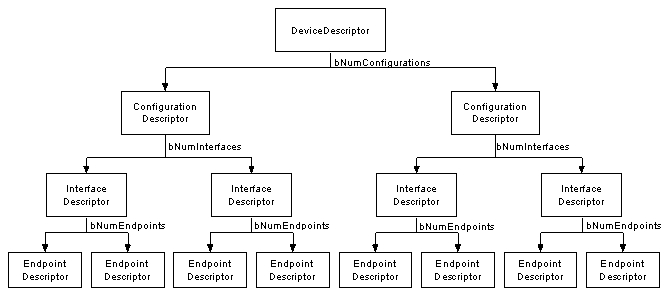
\includegraphics[width=0.7\textwidth]{./descr.jpg}
		\caption{Descriptor architecture}
		\label{Descriptor architecture}
\end{figure}

A typical enumeration follows:
\begin{packed_item}
	\item \textbf{GET\_DEVICE\_DESCRIPTOR}: The host sends a get device descriptor request. The device
replies with its device descriptor to report its attributes (Device Class, maximum packet size for endpoint zero)
	\item \textbf{SET\_ADDRESS}: A USB device uses the default address (0) after reset until the host assigns a unique address using the set address request. The firmware writes the device address assigned by the host
	\item \textbf{GET\_CONFIGURATION\_DESCRIPTOR}: The host sends a get configuration request. The device replies with its configuration descriptor, interface descriptor and endpoint descriptor. The configuration descriptor describes the number of interfaces provided by the configuration, the power source
(Bus or Self powered) and the maximum power consumption of the USB device from the bus.
The Interface descriptor describes the number of endpoints used by this interface. The Endpoint
descriptor describes the transfer type supported and the bandwidth requirements
	\item \textbf{SET\_CONFIGURATION}: The host assigns a configuration value to the device based on the
configuration information. The device is now configured and ready to be used
\end{packed_item}


\subsection{USB 2.0 transactions}
A transfer consists of one or more transactions. Each transaction contains a token packet and may contain a data and/or handshake packet.

\begin{figure}[h!]
		\centering
		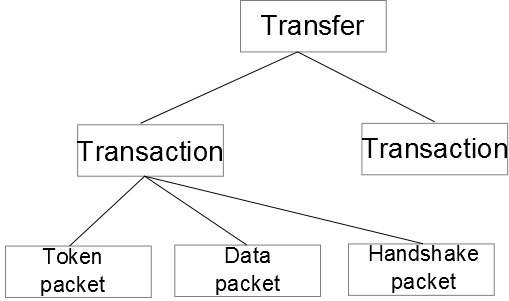
\includegraphics[width=0.4\textwidth]{./transfer.jpg}
		\caption{USB 2.0 transaction}
		\label{USB 2.0 transaction}
\end{figure}

I will illustrate a whole transfer with a control read transfer. This type of transfer is used by the host to request descriptors to a device on the control endpoint:
\begin{packed_item}
	\item \textbf{Setup transaction}:
	\begin{packed_item}
		\item SETUP token packet sent by the host
		\item Data packet: the host sends a request concerning specific descriptor
		\item Handshake packet: the device returns ACK
	\end{packed_item}
	
	\item \textbf{One or more data transaction(s)}:
	\begin{packed_item}
		\item IN token packet sent by the host
		\item Data packet: the device sends the descriptor requested
		\item Handshake packet sent by the host
	\end{packed_item}
	
	
	\item \textbf{Status transaction}:
	\begin{packed_item}
		\item OUT token packet sent by the host
		\item Data packet: 0 length data
		\item Handshake packet: the device returns the status
	\end{packed_item}
	
\end{packed_item}


Concerning bulk or interrupts endpoints, a whole OUT transfer can be:
\begin{packed_item}
	\item \textbf{OUT transaction}:
	\begin{packed_item}
		\item OUT token packet sent by the host
		\item Data packet: the host sends data
		\item Handshake packet: the device returns the status (ACK, NAK or STALL)
	\end{packed_item}
\end{packed_item}

Isochronous transfers are the same as bulk or interrupt transfers without the handshake packet. Occasional errors must be acceptable on isochronous transfers.



\newpage
\section{USB Device stack}
A USB device stack has been developed to allow mbed users to design their own USB device or to use their mbed to emulate a USB peripheral such as a keyboard or a mouse. I did not implemented the USB device stack from scratch but I had low level layers developed in a previous project. I added some functionnalities to these low layers to support for instance all kinds of endpoints and implemented several USB classes:
\begin{packed_item}
	\item HID (Human Interface Device)
	\item MSD (Mass Storage Device)
	\item Audio
	\item MIDI
	\item a subset of CDC (Communication Device Class) to provide a virtual serial port
\end{packed_item}

USB defines class code information that is used to identify a device�'s functionality. This class code is parsed by the USB host stack to load an appropriate device driver.

\begin{figure}[h!]
		\centering
		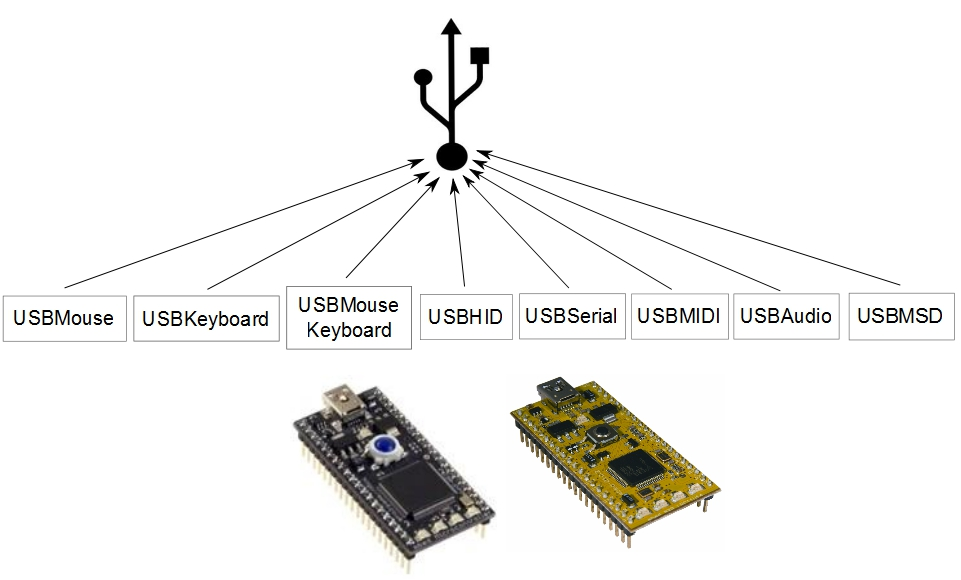
\includegraphics[width=0.7\textwidth]{./usb_capa1.jpg}
		\caption{USB device stack capabilities}
		\label{USB device stack capabilities}
\end{figure}

I will describe in this section the USB stack architecture and some USB classes such as HID, MSD, Audio and CDC.


\subsection{USB Device stack architecture}
\begin{figure}[h!]
		\centering
		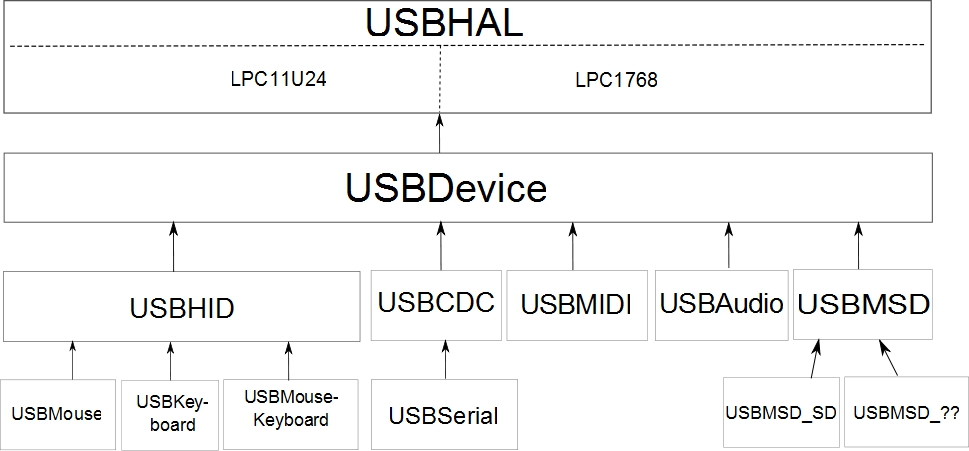
\includegraphics[width=0.7\textwidth]{./usb_arch3.jpg}
		\caption{USB device stack architecture}
		\label{USB device stack architecture}
\end{figure}

\begin{packed_item}

	\item \textbf{USBHAL}: The USB hardware layer for the LPC11U24 and for the LPC1768. In this class, all low level methods are defined. There are USBHAL\_LPC11U24.cpp and USBHAL\_LPC1768.cpp which define functions defined in USBHAL.h. The right .cpp file is chosen according to a macro defined by the compiler: if a user is compiling a program for the LPC1768, the macro TARGET\_LPC1768 is defined. If a user wants to compile a program for the LPC11U24, the macro TARGET\_LPC11U24 is defined. Virtual functions are called on specific events to be treated by subclasses
	
	\item \textbf{USBDevice}: This layer is in charge of abstracting the hardware. At this level, no differences are made between the LPC11U24 and the LPC1768 concerning the target. USBDevice is in charge of performing the setup packet treatment (enumeration step is performed in this class) and provide an abstraction to handle the USB interface

	\item \textbf{USB class layer}:
		\begin{packed_item}
			\item USBHID: implements standard requests of the HID class specification. When a USBHID object is instantiated, the mbed is enumerated as a generic HID device so that raw data can be sent and received to and from a custom program running on the host side
			\item USBCDC: implements a subset of the CDC class specification to allow the mbed to be recognized as a virtual serial port
			\item USBMIDI: enables the mbed to send and receive MIDI messages to and from a computer
			\item USBAudio: implements standard requests of the USB Audio class. The mbed is enumerated as a microphone and a speaker on the same device
			\item USBMSD: implements the mass storage specification. This class is generic: a subclass has to implement some pure virtual functions defined in USBMSD to access a storage chip
		\end{packed_item}
		
	\item \textbf{USB device layer}:
		\begin{packed_item}
			\item USBMouse: used to emulate a mouse
			\item USBKeyboard: used to emulate a keyboard
			\item USBMouseKeyboard: used to emulate a mouse and a keyboard at the same time
			\item USBSerial: used to emulate a virtual serial port
			\item USBMSD\_??: All users can implement their own class which inherits from USBMSD in order to access their storage chip
		\end{packed_item}
	
\end{packed_item}


\subsection{USBHAL: USB Hardware abstraction layer for the LPC11U24}
This section describes the hardware layer implemented for the mbed LPC11U24. This microcontroller has a built-in USB 2.0 device controller. It also has 2 kB of RAM dedicated for USB operations.

\begin{figure}[h!]
		\centering
		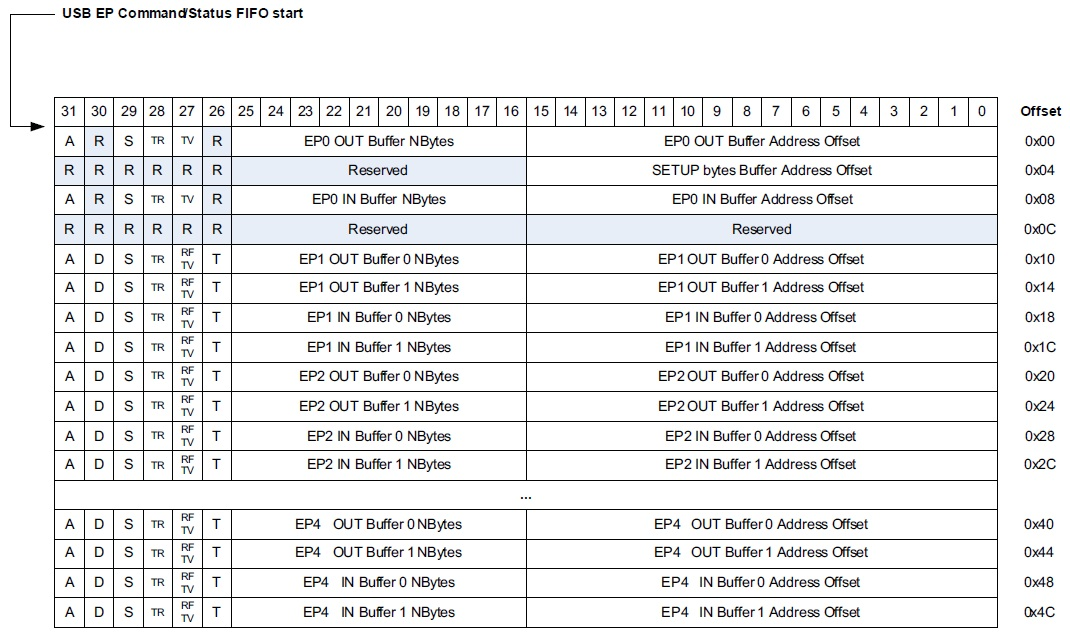
\includegraphics[width=0.9\textwidth]{./usb_endpoints.jpg}
		\caption{USB endpoints status array}
		\label{USB endpoints status array}
\end{figure}

To describe the state of each endpoints available, we need to allocate space in USB RAM as specified in the previous figure. Main fields of endpoints status array are:
\begin{packed_item}
	\item A: the endpoint is active or not
	\item NBytes: For OUT endpoints this is the number of bytes that can be received in this buffer. For IN endpoints this is the number of bytes that must be transmitted
	\item Address offset: represents the end of the address where will be stored data. The beginning of the address is specified in DATABUFSTART register 
\end{packed_item}



Main methods for USBHAL class ARE:

\begin{packed_item}
	\item Memory allocation for endpoints status list and endpoint 0 buffers. These initializations are done in the constructor of USBHAL::USBHAL
	\item Space allocation is required To add more endpoints. This is done in the method: USBHAL::realiseEndpoint
	\item To read a specific endpoint:
		\begin{packed_item}
			\item Fill the endpoint status list (active bit, address offset and NBytes). After this step, the endpoint is ready to receive data. This is done in USBHAL::endpointRead
			\item When a data is received on the specific endpoint, an interrupt is raised. Software can read data in the buffer of this OUT endpoint. This is done in USBHAL::endpointReadResult
		\end{packed_item}
	\item To write on a specific endpoint:
		\begin{packed_item}
			\item Fill the endpoint status list (active bit, address offset and NBytes). Copy data in the buffer of the IN endpoint. After this step, the endpoint is ready to send data. This is done in USBHAL::endpointWrite
			\item Wait until the writing has been effectively done. This is done in USBHAL::endpoint-\\WriteResult
		\end{packed_item}
\end{packed_item}


When a specific event occurs, USBHAL calls virtual functions which can be overrided in a subclass to perform a custom treatment. Main callback functions are:
\begin{packed_item}
	\item SOF(int frameNumber): called on each Start Of Frame event (each millisecond)
	\item EP0setupCallback(): called when a setup packet is received
	\item EPx\_OUT\_callback(): called a data has been received on a specific endpoint
	\item EPx\_IN\_callback(): called when a data has been sent on a specific endpoint
\end{packed_item}

These callback methods are called from the USB interrupt handler:

\begin{lstlisting}[label=Main part of the USB interrupt handler,caption=Main part of the USB interrupt handler]
void USBHAL::usbisr(void) {
    // Start of frame
    if (LPC_USB->INTSTAT & FRAME_INT) {
        // Clear SOF interrupt
        LPC_USB->INTSTAT = FRAME_INT;

        // SOF event, read frame number
        SOF(FRAME_NR(LPC_USB->INFO));
    }

    // Endpoint 0
    if (LPC_USB->INTSTAT & EP(EP0OUT)) {
        // Clear EP0OUT/SETUP interrupt
        LPC_USB->INTSTAT = EP(EP0OUT);

        // Check if SETUP
        if (LPC_USB->DEVCMDSTAT & SETUP) {

            // Clear EP0IN interrupt
            LPC_USB->INTSTAT = EP(EP0IN);

            // Clear SETUP (and INTONNAK_CI/O) in device status register
            LPC_USB->DEVCMDSTAT = devCmdStat | SETUP;

            // EP0 SETUP event (SETUP data received)
            EP0setupCallback();
        } else {
            // EP0OUT ACK event (OUT data received)
            EP0_OUT_callback();
        }
    }

    if (LPC_USB->INTSTAT & EP(EP0IN)) {
        // Clear EP0IN interrupt
        LPC_USB->INTSTAT = EP(EP0IN);

        // EP0IN ACK event (IN data sent)
        EP0_IN_callback();
    }

    if (LPC_USB->INTSTAT & EP(EP1IN)) {
        // Clear EP1IN interrupt
        LPC_USB->INTSTAT = EP(EP1IN);
        epComplete |= EP(EP1IN);
        if (EP1_IN_callback())
            epComplete &= ~EP(EP1IN);
    }

    if (LPC_USB->INTSTAT & EP(EP1OUT)) {
        // Clear EP1OUT interrupt
        LPC_USB->INTSTAT = EP(EP1OUT);
        epComplete |= EP(EP1OUT);
        if (EP1_OUT_callback())
            epComplete &= ~EP(EP1OUT);
    }
    
    // Same for all following endpoints
    .
    .
    .
}\end{lstlisting}


\subsection{USBDevice: target abstraction and setup packet processing}
\subsubsection{Target abstraction}
One of the purposes of this class is to provide an API in order to handle the USB interface easily:
\begin{packed_item}
	\item init() to initialize the USB controller
	\item connect() to connect a device
	\item disconnect() to disconnect a device
	\item addEndpoint(int endpoint) to add a specific endpoint
	\item readEP(int endpoint) to read a specific endpoint
	\item writeEP(int endpoint) to write a specific endpoint 
\end{packed_item}

\subsubsection{Setup packet processing}
Two data structures has been defined in order to perform the control endpoint processing. The enumeration step is part of this treatment:
\begin{packed_item}
	\item SETUP\_PACKET: to describe a setup packet
	\item CONTROL\_TRANSFER: to describe a transfer on the control endpoint
\end{packed_item}


\begin{lstlisting}[label=Data structures for control endpoint processing,caption=Data structures for control endpoint processing]
typedef struct {
    struct {
        uint8_t dataTransferDirection;
        uint8_t Type;
        uint8_t Recipient;
    } bmRequestType;
    uint8_t  bRequest;
    uint16_t wValue;
    uint16_t wIndex;
    uint16_t wLength;
} SETUP_PACKET;

typedef struct {
    SETUP_PACKET setup;
    uint8_t * ptr;      // pointer on a buffer to be sent
    uint32_t remaining; // remaining bytes on the transfer
    uint8_t direction;  // direction: host > device or device > host
    bool zlp;           // zero length packet
    bool notify;
} CONTROL_TRANSFER;
\end{lstlisting}

\begin{figure}[h!]
		\centering
		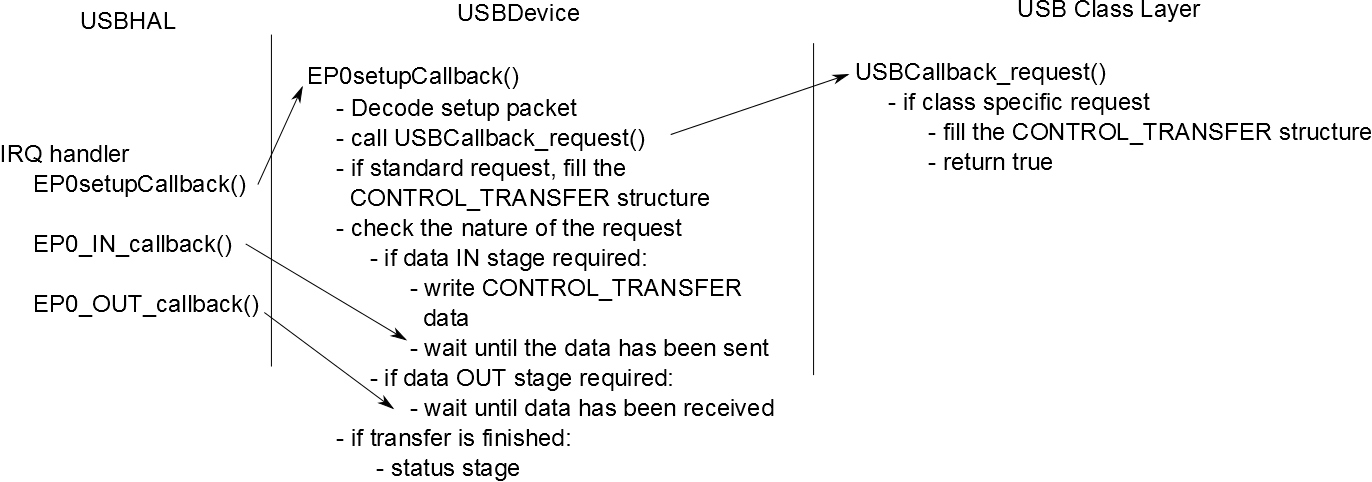
\includegraphics[width=0.9\textwidth]{./setup_packets.jpg}
		\caption{Setup packets processing}
		\label{Setup packets processing}
\end{figure}

For instance, a GET\_DEVICE\_DESCRIPTOR request is processed according to this scheme:
\begin{packed_item}
	\item Reception of a setup packet
	\item Decoding the setup in the SETUP\_PACKET structure
	\item This is not a class specific request so the treatment is done in USBDevice class
	\item The request is GET\_DEVICE\_DESCRIPTOR:
	\begin{packed_item}
		\item Fill the CONTROL\_TRANSFER structure containing in particular a pointer to the device descriptor
		\item This request needs DATA IN stages (the device needs to send the descriptor)
		\item Send data until CONTROL\_TRANSFER.remaining == 0
		\item Read the control endpoint for the status transaction
	\end{packed_item}
\end{packed_item}


A basic device descriptor is quite common for USB devices. Importants fields are:
\begin{packed_item}	
	\item bcdUSB which is the USB specification release number
	\item bDeviceClass specifies the device class
	\item bMaxPacketSize0 specifies the maximum packet size for endpoint 0
\end{packed_item}

\begin{lstlisting}[label=Device Descriptor,caption=Device Descriptor]
uint8_t * USBDevice::deviceDesc() {
    static uint8_t deviceDescriptor[] = {
        DEVICE_DESCRIPTOR_LENGTH,       // bLength 
        DEVICE_DESCRIPTOR,              // bDescriptorType 
        LSB(USB_VERSION_2_0),           // bcdUSB (LSB) 
        MSB(USB_VERSION_2_0),           // bcdUSB (MSB) 
        0x00,                           // bDeviceClass 
        0x00,                           // bDeviceSubClass 
        0x00,                           // bDeviceprotocol 
        MAX_PACKET_SIZE_EP0,            // bMaxPacketSize0 
        LSB(VENDOR_ID),                 // idVendor (LSB) 
        MSB(VENDOR_ID),                 // idVendor (MSB) 
        LSB(PRODUCT_ID),                // idProduct (LSB) 
        MSB(PRODUCT_ID),                // idProduct (MSB) 
        LSB(PRODUCT_RELEASE),           // bcdDevice (LSB) 
        MSB(PRODUCT_RELEASE),           // bcdDevice (MSB) 
        STRING_OFFSET_IMANUFACTURER,    // iManufacturer 
        STRING_OFFSET_IPRODUCT,         // iProduct 
        STRING_OFFSET_ISERIAL,          // iSerialNumber 
        0x01                            // bNumConfigurations 
    };
    return deviceDescriptor;
}
\end{lstlisting}

\subsection{USBHID class}
\subsubsection{Introduction}
HID is one of the most frequently used USB classes. The HID class was primarily defined for devices that are used by humans to control the operation of computer systems. Typical examples of HID devices include keyboards, mice, trackballs, and joysticks. HID devices may have knobs, switches, buttons, sliders, etc. The HID class is also frequently used for devices that may not require human interaction but provide data in a similar format to HID class devices. Since all operating systems have a built-in HID driver, it's easy to design a USB HID device which doesn't require any specific driver.

Data exchanged between the host and device resides in a structure called reports. The report format is flexible and can handle any format of data, but each report has a fixed size. This size is specified in a HID descriptor which is transmitted as part of the configuration descriptor.
HID devices are required to provide a Report Descriptor which enumerates all data fields of a report. A HID device can have at most one interrupt IN endpoint and one interrupt OUT endpoint (and the control endpoint to perform the enumeration step).

For each field in the report, the Report Descriptor defines how many bits the field consumes, how often this data is repeated, and which is the type of the data field. Thus, report descriptors are specific to a device.
\\

\begin{lstlisting}[label=HID Configuration Descriptor,caption=HID Configuration Descriptor]
uint8_t * USBHID::configurationDesc() {
    static uint8_t configurationDescriptor[] = {
        CONFIGURATION_DESCRIPTOR_LENGTH,// bLength
        CONFIGURATION_DESCRIPTOR,       // bDescriptorType
        LSB(TOTAL_DESCRIPTOR_LENGTH),   // wTotalLength (LSB)
        MSB(TOTAL_DESCRIPTOR_LENGTH),   // wTotalLength (MSB)
        0x01,                           // bNumInterfaces
        DEFAULT_CONFIGURATION,          // bConfigurationValue
        0x00,                           // iConfiguration
        C_RESERVED | C_SELF_POWERED,    // bmAttributes
        C_POWER(0),                     // bMaxPower

        //Interface descriptor
        INTERFACE_DESCRIPTOR_LENGTH,    // bLength
        INTERFACE_DESCRIPTOR,           // bDescriptorType
        0x00,                           // bInterfaceNumber
        0x00,                           // bAlternateSetting
        0x02,                           // bNumEndpoints
        HID_CLASS,                      // bInterfaceClass
        HID_SUBCLASS_NONE,              // bInterfaceSubClass
        HID_PROTOCOL_NONE,              // bInterfaceProtocol
        0x00,                           // iInterface

        //hid descriptor
        HID_DESCRIPTOR_LENGTH,          // bLength
        HID_DESCRIPTOR,                 // bDescriptorType
        LSB(HID_VERSION_1_11),          // bcdHID (LSB)
        MSB(HID_VERSION_1_11),          // bcdHID (MSB)
        0x00,                           // bCountryCode
        0x01,                           // bNumDescriptors
        REPORT_DESCRIPTOR,              // bDescriptorType
        LSB(reportDescLength()),  			// wDescriptorLength (LSB)
        MSB(reportDescLength()),  			// wDescriptorLength (MSB)

        //endpoint descriptor (interrupt IN endpoint)
        ENDPOINT_DESCRIPTOR_LENGTH,     // bLength
        ENDPOINT_DESCRIPTOR,            // bDescriptorType
        PHY_TO_DESC(EPINT_IN),          // bEndpointAddress
        E_INTERRUPT,                    // bmAttributes
        LSB(MAX_PACKET_SIZE_EPINT),     // wMaxPacketSize (LSB)
        MSB(MAX_PACKET_SIZE_EPINT),     // wMaxPacketSize (MSB)
        1,                              // bInterval (milliseconds)

        //endpoint descriptor (interrupt OUT endpoint)
        ENDPOINT_DESCRIPTOR_LENGTH,     // bLength
        ENDPOINT_DESCRIPTOR,            // bDescriptorType
        PHY_TO_DESC(EPINT_OUT),         // bEndpointAddress
        E_INTERRUPT,                    // bmAttributes
        LSB(MAX_PACKET_SIZE_EPINT),     // wMaxPacketSize (LSB)
        MSB(MAX_PACKET_SIZE_EPINT),     // wMaxPacketSize (MSB)
        1,                              // bInterval (milliseconds)
    };
    return configurationDescriptor;
}
\end{lstlisting}

In the configuration descriptor, we find the interface descriptor which defines the class used by this device (HID\_CLASS) and the number of endpoints that will be used (2). The HID descriptor gives information on the length of the report descriptor. Finally, there are endpoint descriptors. The communication uses two interrupt endpoints: one IN to send data to the host and one OUT to receive data from the host. Interrupts endpoint are polled by the host, that is why there is a bInterval field in endpoint descriptors.
\\


\subsubsection{HID: Class specific requests}
The HID specification defines several class specific requests. All these requests are processed in the USBCallback\_request() virtual method. The main specific requests are:
\begin{packed_item}
	\item GET\_REPORT: allows the host to receive a report via the Control pipe. This request is useful at initialization time for absolute items and for 
determining the state of feature items
	\item SET\_REPORT: allows the host to send a report to the device, possibly setting the state of input, output, or feature controls.
	\item GET\_DESCRIPTOR: to request the HID descriptor and the report descriptor
\end{packed_item}

\subsubsection{Generic HID device}
If a USBHID is instantiated, the device created is a generic HID device. This means that it is not a specific device such as a mouse or a keyboard but a device which can send and receive raw data. The report descriptor for this device is:
 
\begin{lstlisting}[label=Generic HID Report Descriptor,caption=Generic HID Report Descriptor]
uint8_t * USBHID::reportDesc() {
    static uint8_t reportDescriptor[] = {
        0x06, LSB(0xFFAB), MSB(0xFFAB),
        0x0A, LSB(0x0200), MSB(0x0200),
        0xA1, 0x01,         // Collection 0x01
        
        //data are sent in packets containing input_length bytes
        0x75, 0x08,         // report size = 8 bits
        0x15, 0x00,         // logical minimum = 0
        0x26, 0xFF, 0x00,   // logical maximum = 255
        0x95, input_length, // report count
        0x09, 0x01,         // usage
        0x81, 0x02,         // Input (array)
        
        //data are received in packets containing output_length bytes
        0x95, output_length,// report count
        0x09, 0x02,         // usage
        0x91, 0x02,         // Output (array)
        
        0xC0                // end collection

    };
    return reportDescriptor;
}
\end{lstlisting}

There are two main parts:
\begin{packed_item}
	\item Bytes are sent to the host by packets of length \textbf{input\_length}
	\item Bytes are received by packets of length \textbf{output\_length}
\end{packed_item}


Additionnally, this class defines methods to send and receive reports:

\begin{lstlisting}[label=Send and receive HID reports,caption=Send and receive HID reports]
bool USBHID::send(HID_REPORT *report)
{
    return USBDevice::writeEP(EPINT_IN, report->data, report->length, MAX_HID_REPORT_SIZE);
}


bool USBHID::read(HID_REPORT *report)
{
    uint16_t bytesRead = 0;
    bool result;
    result = USBDevice::readEP(EPINT_OUT, report->data, &bytesRead, MAX_HID_REPORT_SIZE);
    if(!readStart(EPINT_OUT, MAX_HID_REPORT_SIZE))
        return false;
    report->length = bytesRead;
    return result;
}
\end{lstlisting}

\subsubsection{USBMOUSE}
USBMOUSE class is a subclass of USBHID. The important descriptor of this class is the report descriptor which defines data structures which will be exchanged.


\begin{lstlisting}[label=Mouse Report Descriptor,caption=Mouse Report Descriptor]
uint8_t * USBMouse::reportDesc() {
    static uint8_t reportDescriptor[] = {
        USAGE_PAGE(1),      0x01,       // Generic Desktop
        USAGE(1),           0x02,       // Mouse
        COLLECTION(1),      0x01,       // Application
        USAGE(1),           0x01,       // Pointer
        COLLECTION(1),      0x00,       // Physical

        // Buttons
        REPORT_COUNT(1),    0x03,       // 3 buttons
        REPORT_SIZE(1),     0x01,       // 1 bit for each button
        USAGE_PAGE(1),      0x09,       // Buttons
        USAGE_MINIMUM(1),   0x1,    
        USAGE_MAXIMUM(1),   0x3,
        LOGICAL_MINIMUM(1), 0x00,       // Button not pressed
        LOGICAL_MAXIMUM(1), 0x01,       // Button pressed
        INPUT(1),           0x02,       // Input, absolute data
        REPORT_COUNT(1),    0x01,       // Padding to fill 1 byte (5 + 3)
        REPORT_SIZE(1),     0x05,
        INPUT(1),           0x01,
        
        // X, Y and scroll
        REPORT_COUNT(1),    0x03,       // 3 features: X, Y, scroll
        REPORT_SIZE(1),     0x08,       // 1 byte for X, 1 byte for Y and 1 byte for scroll
        USAGE_PAGE(1),      0x01,
        USAGE(1),           0x30,       // X
        USAGE(1),           0x31,       // Y
        USAGE(1),           0x38,       // scroll
        LOGICAL_MINIMUM(1), 0x81,       // Minimum: -127
        LOGICAL_MAXIMUM(1), 0x7f,       // Maximum: 127
        INPUT(1),           0x06,       // Input, Relative data

        END_COLLECTION(0),
        END_COLLECTION(0),
    };
    return reportDescriptor;
}
\end{lstlisting}

On this report descriptor, we can distinguish three different parts:
\begin{packed_item}
	\item At the beginning, there is the indication that a mouse report descriptor will be described
	\item Mouse buttons: There are 3 buttons represented by 1 bit. Values for these buttons are 0 or 1 (pressed or not). They are input values which means that the device will send information to the host
	\item X, Y and scroll: 3 different features, each represented by 1 byte. Values can vary between -127 and 127. They are also input values
\end{packed_item}

The main method to send a mouse state to the host is:

\begin{lstlisting}[label=Mouse Report Descriptor,caption=Mouse Report Descriptor]
bool USBMouse::mouseSend(int8_t x, int8_t y, uint8_t buttons, int8_t z) {
    HID_REPORT report;
    report.data[0] = buttons & 0x07;
    report.data[1] = x;
    report.data[2] = y;
    report.data[3] = -z; // >0 to scroll down, <0 to scroll up

    report.length = 4;

    return USBHID::send(&report);
}
\end{lstlisting}

Concerning USBKeyboard and USBMouseKeyboard classes, the important part is the definition of the report descriptor which defines the format of data sent to the host. 



\subsection{CDC class to emulate a virtual serial port}
\subsubsection{Introduction}
The Communication Device Class (CDC) is a general-purpose way to enable all
types of communications on the Universal Serial Bus. This class makes it possible
to connect telecommunication devices such as digital telephones or analog
modems, as well as networking devices such as ADSL or Cable modems.
While a CDC device enables the implementation of quite complex devices, it can also
be used as a very simple solution for communication on the USB. For example, a CDC
device can appear as a virtual COM port, which greatly simplifies application programming
on the host side. For mbed a subset of the CDC class has been implemented in order to create
a virtual serial port over USB.

\subsubsection{Descriptors}
Concerning the device descriptor, bDeviceClass has to be 02h to specify a CDC device.\\


Two interfaces are used in the configuration descriptor:
\begin{packed_item}
	\item \textbf{Communication Class Interface}: used to request and manage the device state. This interface is also used by the host to request capabilities and parameters of the communication. To provide information about the communication, four descriptors are used:
	\begin{packed_item}
		\item CDCHeaderDescriptor: marks the beginning of the concatenated set of functional descriptors for the interface
		\item CDCCallManagementDescriptor: describes the processing of calls for the Communication Class interface
 		\item CDCAbstractControlManagementDescriptor: describes the commands supported by the Communication Class interface. This device supports for instance the request GET\_LINE\_CODING which allows the host to know parameters of the communication (number of stop bits, parity, number of data bits)
		\item CDCUnionDescriptor: describes the relationship between a group of interfaces that can be considered to form
a functional unit. Here, the master interface is the Communication Class Interface and the slave one is the data Class Interface
	\end{packed_item}
	\item \textbf{Data Class Interface}: this interface is used for data transfers. For the communication, either bulk or interrupt endpoints are required. For a serial port,  reliability
of the transmission is very important and the data transfers are not time-critical. That is why, two bulk endpoints (one IN and one OUT) are used
\end{packed_item}


\subsubsection{CDC: Class specific requests}
The CDC specification defines several class specific requests. All these requests are processed in the USBCallback\_request() virtual method. The main specific requests are:
\begin{packed_item}
	\item GET\_LINE\_CODING: allows the host to know parameters of the communication (number of stop bits, parity, number of data bits)
	\item SET\_LINE\_CODING: allows the host to specify typical line-character formatting properties
\end{packed_item}

\subsubsection{USBSerial class}
Once the device is enumerated, data can be exchanged over the two bulk endpoints. To send a character, we just write the character on the bulk IN endpoint. Characters received are pushed on a circular buffer called buf. This step is done in the EPx\_OUT\_callback() virtual function called when a packet is received. We can then define two methods to send and receive data:

\begin{lstlisting}[label=USBSerial: putc and getc,caption=USBSerial: putc and getc]
int USBSerial::_putc(int c) {
		writeEP(EPBULK_IN, uint8_t *)&c, 1, MAX_CDC_REPORT_SIZE)
    return 1;
}

int USBSerial::_getc() {
    uint8_t c;
    while (buf.isEmpty());
    buf.dequeue(&c);
    return c;
}

bool USBSerial::EP2_OUT_callback() {
    uint8_t c[65];
    uint16_t size = 0;

    //we read the packet received and put it on the circular buffer
    readEP(EPBULK_OUT, c, size, MAX_CDC_REPORT_SIZE)
    for (int i = 0; i < size; i++) {
        buf.queue(c[i]);
    }

    //call a potential handler
    rx.call();

    // We reactivate the endpoint to receive next characters
    readStart(EPBULK_OUT, MAX_PACKET_SIZE_EPBULK);
    return true;
}
\end{lstlisting}




\subsection{MSD class}
\subsubsection{Introduction}
The Mass Storage Device (MSD) class is an extension to the USB specification that defines
how mass storage devices, such as a hard-disk, SD card or flash chip should operate on the USB.
Many devices use the MSD class to simplify data transfer. More common devices which use this class are hard-drives, USB-stick, MP3 or video player.

\subsubsection{MSD descriptors}
The MSD configuration descriptor defines one interface with bInterfaceClass = 08h specifying the mass storage class. Two bulk endpoints are then defined to transfer data. Bulk endpoints are used because large amount of data can be transferred.

\subsubsection{MSD class specific requests}
The MSD specification defines several class specific requests. All these requests are processed in the USBCallback\_request() virtual method. The main specific requests are:
\begin{packed_item}
	\item RESET: used to reset the device by the host
	\item GET\_MAX\_LUN: allows the host to determine the maximum Logical Unit Number (LUN) supported by the device. This is not equivalent to the number of logical unit on the device, since units are numbered starting from 0. In the mbed library, only 1 logical unit is supported.
\end{packed_item}

\subsubsection{MSD transaction}
The communication between the device and the host is divided into three steps:
\begin{packed_item}
	\item Command stage
	\item An optional data stage
	\item Status stage
\end{packed_item}

The \textbf{command stage} is used by the host to transmit instructions to be performed by the device. These instructions are contained in a Command Block Wrapper (CBW) sent by the host. The CBW describes several parameters of the transaction:

\begin{table}[h!]
\centering
\begin{tabular}{|c|c|c| >{\arraybackslash}m{9cm} |}
\hline

Offset & Field & Length (bytes) & Meaning \\ \hline
0 & dCBWSignature & 4 & Signature to identify a valid CBW (0x43425355) \\ \hline
4 & dCBWTag & 4 &  id of the CBW. The device have to answer in the status stage by sending a Command Status Wrapper (CSW) containing the same id. \\ \hline
8 & dCBWTransferLength & 4 & Length of transfer \\ \hline
12 & bmCBWFlags & 1 & bit7: transfer direction (0: OUT, 1: IN) \\ \hline
13 & bCBWLUN & 1 & \textbf{Bits 0-3}: logical unit to which the command is sent \\ \hline
14 & bCBWCBLength & 1 & \textbf{Bits 0-5}: Length of command block in bytes \\ \hline
15 & CBWCB & 0-16 & Command block: instructions to be executed by the device \\ \hline

\end{tabular}
\caption{Command Block Wrapper (CBW)}
\label{Command Block Wrapper (CBW)}
\end{table}

When a CBW has been received and decoded by the device, an optional \textbf{data stage} may take
place if the command requires it. During this step, data flow from or to the device (for instance, if the host wants to read the content of an SD card, there will be a data IN stage). Several transfers can occur successively.
\\

Once the data stage performed, the device must send a Command Status Wrapper (CSW) in response to the CBW. A CSW is used to return the result of a command.

\begin{table}[h!]
\centering
\begin{tabular}{|c|c|c| >{\arraybackslash}m{9cm} |}
\hline

Offset & Field & Length (bytes) & Meaning \\ \hline
0 & dCSWSignature & 4 & Signature to identify a valid CSW (0x53425355) \\ \hline
4 & dCSWTag & 4 &  Same id as in the CBW \\ \hline
8 & dCSWDataResidue & 4 & Difference between expected and real transfer length \\ \hline
12 & bCSWStatus & 1 & Indicates the result (success or failure) of the command. \\ \hline

\end{tabular}
\caption{Command Status Wrapper (CSW)}
\label{Command Status Wrapper (CSW)}
\end{table}

\subsubsection{MSD State machine}
To implement the three previous step of a transaction, a state machine is used.
This state machine contains 5 states:
\begin{packed_item}
	\item WAIT\_CBW: waiting for the reception of a valid CBW. If a non valid CBW is received, send a CSW reporting an error.
	\item PROCESS\_CBW: decode and execute command from the CBW. If there is a processing error, go into the ERROR state
	\item SEND\_CSW: a CSW is sent
	\item WAIT\_CSW: waiting for CSW reception by the host
	\item ERROR: to report an error.
\end{packed_item}

\begin{figure}[h!]
		\centering
		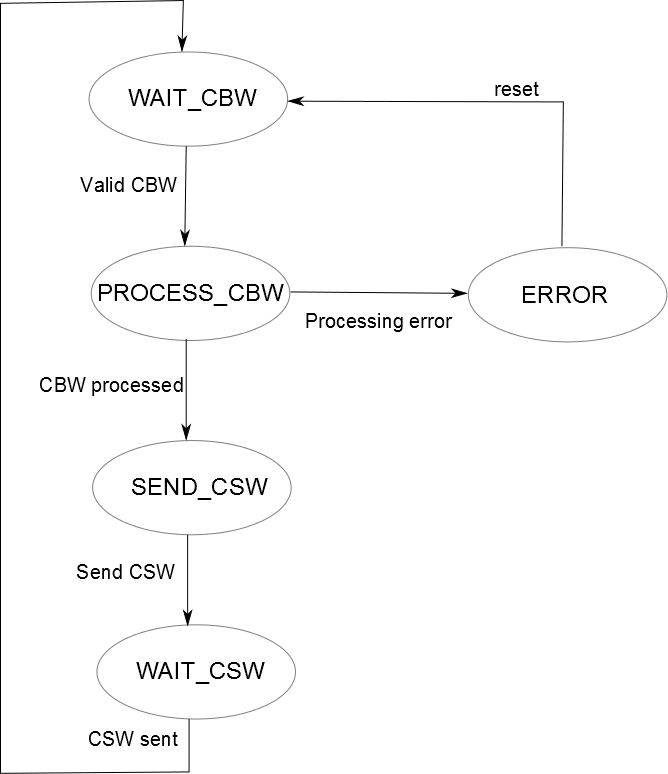
\includegraphics[width=0.5\textwidth]{./msd_state_machine.jpg}
		\caption{MSD state machine}
		\label{MSD state machine}
\end{figure}


\subsubsection{SCSI commands}
All commands sent by the host contained in the CBW are part of the SCSI command architecture. In the SCSI protocol, the initiator sends a SCSI command to the target which then responds. SCSI commands are sent in a block, which consists of a one byte operation code followed by five or more bytes containing command-specific parameters. Upon receiving and processing the CBW the target will return a status code byte.\\


Main commands that have to be processed by the device are:
\begin{packed_item}
	\item SCSI\_INQUIRY: The host usually issues an Inquiry command right after the enumeration phase to get more
information about the device

	\item SCSI\_READ\_CAPACITY: The Read Capacity command enables the host to retrieve the number of blocks present on a
media, as well as their size

	\item SCSI\_READ (6)/(10): This command is used by the host to read data from the device.
	
	\item SCSI\_REQUEST\_SENSE: If there is an error during the execution of a command, the host will issue a
Request Sense to get more information about the problem

	\item SCSI\_TEST\_UNIT\_READY: This command provides a way to check if a logical unit is ready. If the logical unit is not ready, the device reports an error in the CSW. Then the host sends a SCSI\_REQUEST\_SENSE to have more information about the error
\end{packed_item}

The main method to decode a CBW and a SCSI command is:
\begin{lstlisting}[label=MSD CBW decoding,caption=MSD CBW decoding]
void USBMSD::CBWDecode(CBW cbw) {
	if (cbw.Signature == CBW_Signature) {
		csw.Tag = cbw.Tag;
		csw.DataResidue = cbw.DataLength;
		if ((cbw.CBLength <  1) || (cbw.CBLength > 16) ) {
			fail();
		} else {
			switch (cbw.CB[0]) {
				case TEST_UNIT_READY:
					testUnitReady();
					break;
        case REQUEST_SENSE:
          requestSense();
          break;
        case INQUIRY:
          inquiryRequest();
          break;
        case MODE_SENSE6:
          modeSense6();
          break;
        case READ_FORMAT_CAPACITIES:
          readFormatCapacity();
          break;
        case READ_CAPACITY:
          readCapacity();
          break;
        case READ10:
          case READ12:
          if (infoTransfer()) {
            if ((cbw.Flags & 0x80)) {
               stage = PROCESS_CBW;
               memoryRead();
            } else {
               stallEndpoint(EPBULK_OUT);
               csw.Status = CSW_ERROR;
               sendCSW();
            }
          }
          break;
        case WRITE10:
        case WRITE12:
          if (infoTransfer()) {
            if (!(cbw.Flags & 0x80)) {
              stage = PROCESS_CBW;
            } else {
              stallEndpoint(EPBULK_IN);
              csw.Status = CSW_ERROR;
              sendCSW();
            }
          }
          break;
        case VERIFY10:
          if (!(cbw.CB[1] & 0x02)) {
            csw.Status = CSW_PASSED;
            sendCSW();
            break;
          }
          if (infoTransfer()) {
            if (!(cbw.Flags & 0x80)) {
              stage = PROCESS_CBW;
              memOK = true;
            } else {
              stallEndpoint(EPBULK_IN);
              csw.Status = CSW_ERROR;
              sendCSW();
            }
          }
          break;
        default:
          fail();
          break;
      }
   }
}
\end{lstlisting}

\subsubsection{Use of USBMSD with a specific storage chip}
The USBMSD class implements the MSD protocol as defined previously. But this class doesn't work standalone, a subclass is needed to define pure virtual functions called in USBMSD in order to access a specific storage chip.\\


Six pure virtual functions have to be defined:
\begin{packed_item}
	\item virtual \textbf{int disk\_read(char * data, int block)}: function to read a block
	\item virtual \textbf{int disk\_write(const char * data, int block)}: function to write a block
	\item virtual \textbf{int disk\_initialize()}: function to initialize the memory
	\item virtual \textbf{int disk\_sectors()}: return the number of blocks
	\item virtual \textbf{int disk\_size()}: return the memory size
	\item virtual \textbf{int disk\_status()}: return the status of the storage chip (0: OK, 1: not initialized, 2: no medium in the drive, 4: write protection)
\end{packed_item}


\subsection{Audio class}
\subsubsection{Introduction}
The audio class enables a USB device to send and receive, for example, encoded speech or music. In the mbed library, a USB audio device has been developed in order to send and receive audio packets in the same device. An application of the Audio class could be to play music on a speaker or an I2S/I2C chip connected to the mbed, or to send audio packets from a microphone. Devices in the audio class use isochronous transfers for audio streams. Audio devices can either be synchronous or asynchronous:
\begin{packed_item}
	\item Asynchronous isochronous audio endpoints produce or consume data at a rate that is locked either to a
clock external to the USB or to a free-running internal clock. These endpoints cannot be synchronized to a Start Of Frame (SOF)
	\item Synchronous isochronous endpoints are handled in the Start Of Frame event generated each millisecond
\end{packed_item}
In the mbed library, only the synchronous mode has been developed:
\begin{packed_item}
	\item on each Start Of Frame event:
	\begin{packed_item}
		\item if a user has requested the reading of an audio packet: try to read a packet on the OUT isochronous endpoint
		\item if a user wants to send an audio packet: write the audio packet on the IN isochronous endpoint
	\end{packed_item}
\end{packed_item}

\subsubsection{Descriptors}
Three interfaces are defined in the configuration descriptor:
\begin{packed_item}
	\item Audio Control Interface: describes the functional behavior of the device including input terminal, output terminal or features unit:
	\begin{packed_item}
		\item An Input Terminal is used to interface between outside the device and other Units inside the device
		\item An Output Terminal is used to interface between Units inside the audio function and outside the device
		\item A feature Unit provides audio control concerning volume or mute for instance
	\end{packed_item}
	
	\item Audio Streaming Interface: used to interchange digital audio data streams between the Host and the audio device. In our case, two audio streaming interfaces are defined:
	\begin{packed_item}
		\item to receive an audio stream over an isochronous OUT endpoint
		\item to send a stream over an isochronous IN endpoint
	\end{packed_item}
	This interface specifies the type of data exchanged, the number of channels used, the number of bits used to encode a sample or the frequency. In the mbed library, a PCM representation on 16 bits is used to send and receive audio packets. Other parameters can be chosen by the user.
\end{packed_item}

\begin{figure}[h!]
		\centering
		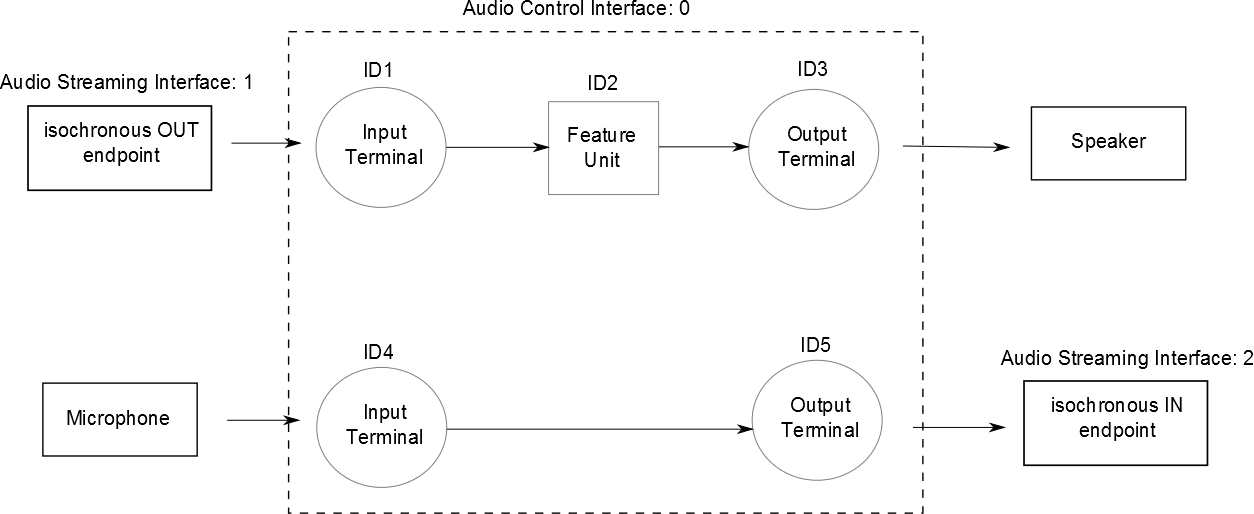
\includegraphics[width=0.8\textwidth]{./audio_archi.jpg}
		\caption{Audio device interfaces}
		\label{Audio device interfaces}
\end{figure}

\subsubsection{Audio class specific requests}
The Audio specification defines several class specific requests. All these requests are processed in the USBCallback\_request() virtual method. Specific requests have been implemented:
\begin{packed_item}
	\item GET\_CUR: allows the host to know the current volume or the mute state
	\item SET\_CUR: allows the host to set the current volume or the mute state
	\item GET\_MIN: allows the host to know the minimum volume level
	\item GET\_MAX: allows the host to know the maximum volume level
	\item GET\_RES: allows the host to know the resolution attribute between two volume levels
\end{packed_item}

\subsubsection{Audio packet management}
As explained before, one audio packet is sent or received on a Start Of Frame event (each millisecond). So let's say that a frequency of 48 kHz has been chosen with 2 channels (stereo). Knowing that each sample of a packet is 16 bits long, 48 * 2 bytes will be received or sent each millisecond for one channel. In total, for 2 channels, 48 * 2 * 2 bytes will be received. The audio length packet received or sent each millisecond can be calculated as:
\begin{center}
	AUDIO\_LENGTH\_PACKET = (FREQ / 500) * nb\_channel
\end{center}

Audio packets have to be interpreted differently, according to the number of channels:

\begin{figure}[h!]
		\centering
		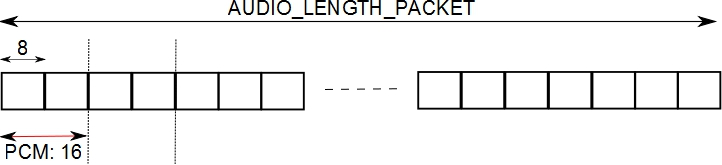
\includegraphics[width=0.7\textwidth]{./pcm.jpg}
		\caption{PCM packet: mono}
		\label{PCM packet: mono}
\end{figure}

\begin{figure}[h!]
		\centering
		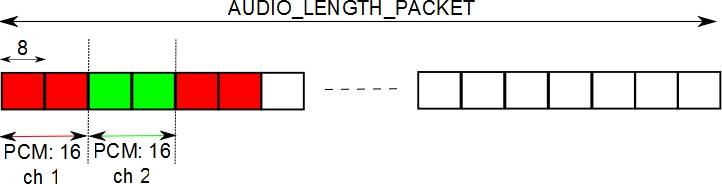
\includegraphics[width=0.7\textwidth]{./pcm_stereo.jpg}
		\caption{PCM packet: stereo}
		\label{PCM packet: stereo}
\end{figure}


The main part for sending and receiving audio packets is in the virtual function called in USBHAL on each Start Of Frame event:
\begin{lstlisting}[label=Audio packets management in SOF events,caption=Audio packets management in SOF events]
// Called in ISR context on each Start Of Frame
void USBAudio::SOF(int frameNumber) {
    uint16_t size = 0;
    
    //read the isochronous endpoint if the user has provided a buffer
    if (buf_stream_in != NULL) {
       if (USBDevice::readEP_NB(EP3OUT, (uint8_t *)buf_stream_in, &size, PACKET_SIZE_ISO_IN)) {
           // if an audio packet is available, notify
           if (size) {
               available = true;
               readStart(EP3OUT, PACKET_SIZE_ISO_IN);
           }
       }
    }
    
    //write if needed
    if (buf_stream_out != NULL) {
       USBDevice::writeNB(EP3IN, (uint8_t *)buf_stream_out, PACKET_SIZE_ISO_OUT, PACKET_SIZE_ISO_OUT);
    }

    SOF_handler = true;
}
\end{lstlisting}

\section{Conclusion}
Mbed users can now use their mbed to emulate a USB device. I really wanted explore all the capabilities of USB. This is why I developed several classes:
\begin{packed_item}
	\item Human Interface Device (HID), in my opinion the best way to develop a custom USB device as it permits the exchange of raw data without the need for a specific driver on the host side.
	\item Communication Device Class (CDC) to provide a virtual serial port
	\item Mass Storage Device (MSD) to access a block storage chip from a computer
	\item Audio to receive and send audio packets
	\item MIDI to send and receive MIDI messages
\end{packed_item}

\chapter*{Conclusion}
By way of conclusion, I again want to thank my manager Simon Ford. He permitted me to explore new domains involved in my projects:
\begin{packed_item}
	\item the Internet of Things project where I had to connect sensors to the Internet over a WebSocket communication. 
	\item the Remote Procedure Call Mechanism over WebSocket which permitted to call methods on a distant mbed
	\item the USB device stack to emulate USB devices with an mbed
\end{packed_item}

The Internet of Things and RPC projects were very interesting because they needed several skills such as:
\begin{packed_item}
	\item software skills in embedded systems to program the mbed
	\item software skills in web programming
	\item hardware skills
\end{packed_item}


Thanks to these projects, I learned a great deal about web programming, in particular Javascript. I am now more familiar with web technologies such as HTML5 and WebSockets. It was very good experience, I found, to develop a project which required several skills. I also really appreciated working on the USB. It was a new domain for me, and it was very interesting to discover all about the USB protocol. It was satisfying and motivating to observe technical results day after day on the USB device stack, knowing that it was a totally new subject for me. In the end, I was happy to be able to provide to mbed users a USB device stack able to emulate many USB classes. \\


This internship has been a great experience. It was a real pleasure to work with the mbed team in a very good atmosphere. Furthermore, carrying out this
internship in a foreign country allowed me to be immersed in a different culture and face the problems asscoiated with living and working entirely with a non-native language (English). I met several
interesting people both in and out of the lab, such as engineers, students, and also people not connected with computer science.




\chapter*{References}
http://www.bbc.co.uk/news/technology-13613536

TODO







\end{document}
